%Talk given at Computational Math Stat Seminar
\documentclass[11pt,compress,xcolor={usenames,dvipsnames},aspectratio=169]{beamer}
%\documentclass[xcolor={usenames,dvipsnames},aspectratio=169]{beamer} %slides and 
%notes
\usepackage{amsmath,datetime,
	mathtools,
	bbm,
	%mathabx,
	array,
	booktabs,
	xspace,
	calc,
	colortbl,
 	graphicx}
\usepackage[usenames]{xcolor}
\usepackage[giveninits=false,backend=biber,style=nature, maxcitenames =10, mincitenames=9]{biblatex}
\addbibresource{FJHown23.bib}
\addbibresource{FJH23.bib}
\usepackage{newpxtext}
\usepackage[euler-digits,euler-hat-accent]{eulervm}
\usepackage{media9}
\usepackage[autolinebreaks]{mcode}

\usetheme{FJHSlimNoFoot169}
\setlength{\parskip}{2ex}
\setlength{\arraycolsep}{0.5ex}

\newcommand{\sol}{S}
\newcommand{\app}{A}
\newcommand{\Sapp}{S_{\textup{app}}}
\newcommand{\LambdaStd}{\Lambda^{\textup{std}}}
\newcommand{\LambdaSer}{\Lambda^{\textup{ser}}}
\newcommand{\LambdaAll}{\Lambda^{\textup{all}}}
\DeclareMathOperator{\spann}{span}
%\DeclareMathOperator{\app}{app}

\providecommand{\HickernellFJ}{H.}


\iffalse
Adaptive Approximation to Multivariate Linear Problems with Inputs Lying in a Cone

Function recovery, differentiation, and integral equations are examples of multivariate problems which require approximate numerical solutions.  One would like to identify a good algorithm, analyze the computational cost to achieve the desired error tolerance, understand how this cost depends on the number of variables, and determine whether the proposed algorithm is nearly optimal relative to the best possible algorithm.  This talk focuses on the situation where the inputs can be represented as series, and where the algorithm is allowed go sample individual series coefficients.  Rather than focusing on inputs lying inside a ball of fixed radius, we focus on inputs lying inside a cone of nice inputs.  This allows us to construct an adaptive algorithm, that automatically determines the number of series coefficients required to achieve the desired error tolerance.  The computational cost of the algorithm is characterized in terms of the space of inputs, space of outputs, solution operator, and definition of the cone.  The information-based complexity of problem and its tractability are also characterized.  These depend on the relative importance of the variables. 
\fi

\renewcommand{\OffTitleLength}{-10ex}
\setlength{\FJHThankYouMessageOffset}{-8ex}
\title{Adaptive Approximation for Multivariate Linear Problems  \\ with Inputs Lying in a Cone}
\author[]{Fred J. Hickernell}
\institute{Department of Applied Mathematics \\
	Center for Interdisciplinary Scientific Computation \\  Illinois Institute of Technology \\
	\href{mailto:hickernell@iit.edu}{\url{hickernell@iit.edu}} \quad
	\href{http://mypages.iit.edu/~hickernell}{\url{mypages.iit.edu/~hickernell}}}

\thanksnote{{\large Joint work with Yuhan Ding, Peter Kritzer, and Simon Mak} \\
	This work partially supported by  NSF-DMS-1522687 and NSF-DMS-1638521 (SAMSI) \& ???
}
\event{RICAM Workshop on Multivariate Algorithms and Information-Based Complexity}
\date[]{\\ November 9, 2018}

\input FJHDef.tex


%Abstract:  When

\newlength{\figwidth}
\setlength{\figwidth}{0.25\textwidth}

\newlength{\figwidthSmall}
\setlength{\figwidthSmall}{0.2\textwidth}

\newcommand{\financePict}{\href{http://i2.cdn.turner.com/money/dam/assets/130611131918-chicago-board-options-exchange-1024x576.jpg}{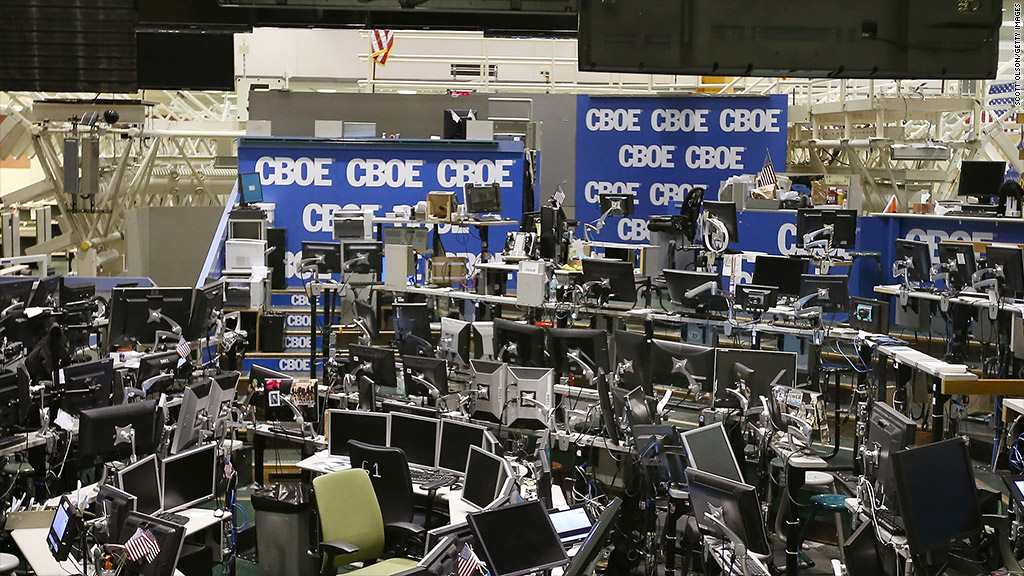
\includegraphics[width
		= 3cm]{ProgramsImages/130611131918-chicago-board-options-exchange-1024x576.jpg}}}
	
	\newcommand{\scoop}[1]{\parbox{#1}{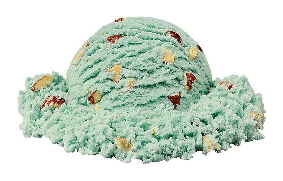
\includegraphics[width=#1]{IceCreamScoop.eps}}\xspace}
	\newcommand{\smallscoop}{\scoop{1cm}}
	\newcommand{\medscoop}{\parbox{1.8cm}{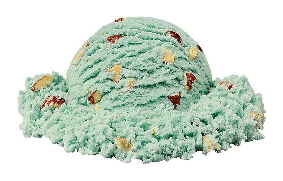
\includegraphics[width=1.8cm]{IceCreamScoop.eps}}\xspace}
	\newcommand{\largescoop}{\scoop{3cm}}
	\newcommand{\ICcone}[1]{\parbox{#1}{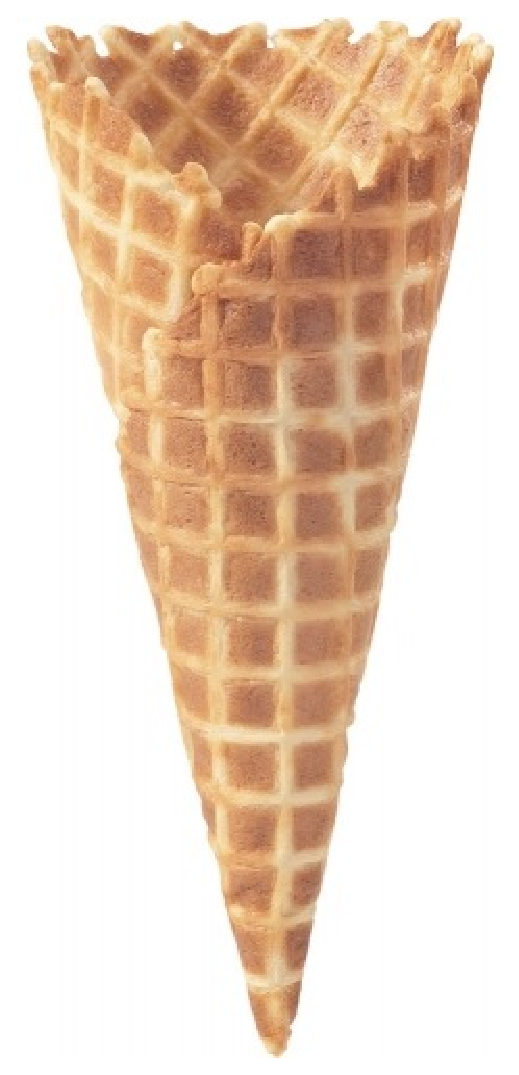
\includegraphics[width=#1,angle=270]{MediumWaffleCone.eps}}\xspace}
	\newcommand{\medcone}{\ICcone{1.2cm}}
	\newcommand{\largercone}{\parbox{2.2cm}{\vspace*{-0.2cm}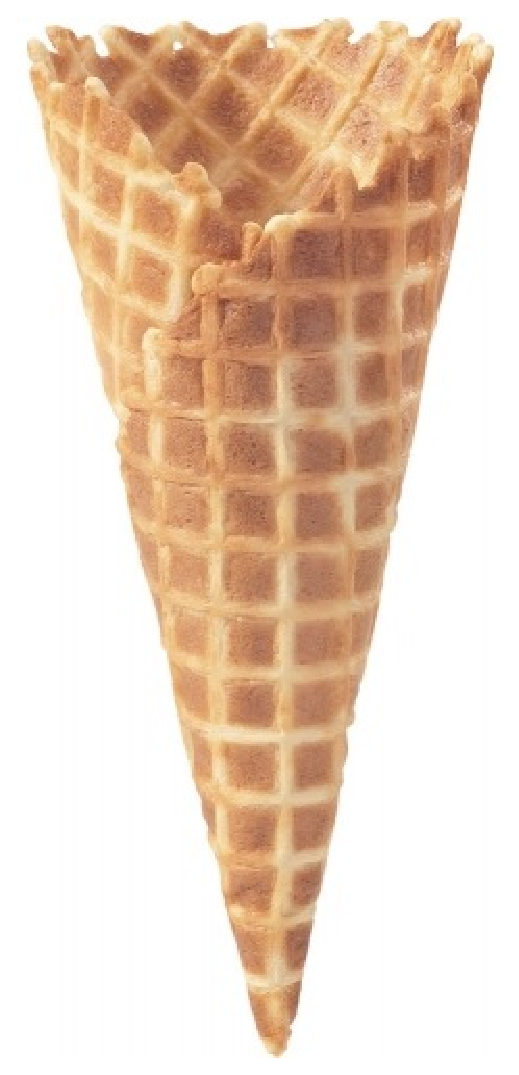
\includegraphics[width=1cm,angle=270]{MediumWaffleCone.eps}}\xspace}
	\newcommand{\largecone}{\ICcone{1.8cm}}
	\newcommand{\smallcone}{\parbox{0.65cm}{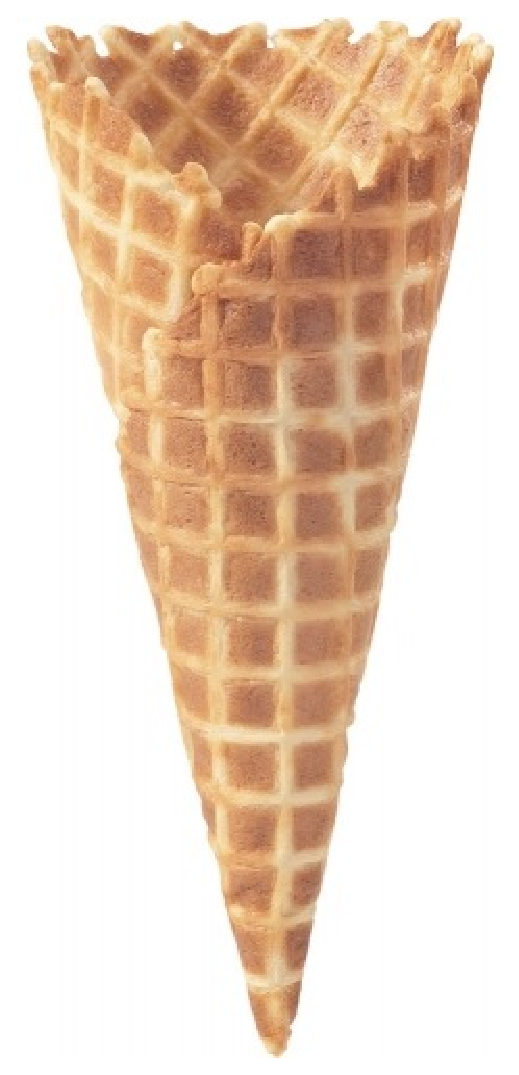
\includegraphics[width=0.3cm,angle=270]{MediumWaffleCone.eps}}\xspace}
	


\begin{document}
\everymath{\displaystyle}
\frame{\titlepage}
\section{Introduction}

\begin{frame}{Multivariate Linear Problems}
\vspace{-3ex}
\begin{tabular}{p{0.47\textwidth}p{0.5\textwidth}}
Given $f \in \cf$ find $S(f) \in \cg$, where \\
$\sol: \cf \to \cg$ is linear, e.g., 
\begin{gather*}
    S(f) = \int_{\reals^d} f(\vx) \, \varrho(\vx) \, \dif \vx\\
    S(f) = f\\
    S(f) = \frac{\partial f}{\partial x_1} \\
    - \nabla^2 S(f) = f, \ \  S(f) = 0 \text{ on boundary}
\end{gather*}
&
\vspace{-7ex}
\alert{Successful algorithms}
\vspace{-3ex}
\begin{multline*}
    \ca(\cc) : = \{\app: \cc \times (0,\infty) \to \cg \text{ such that } \\
\norm[\cg]{\sol(f) - \app(f,\varepsilon) } \le \varepsilon \ \ \forall f \in \cc \subseteq \cf, \ \varepsilon > 0 \}
\end{multline*}

\vspace{-1ex}
where $\app(f,\varepsilon)$ depends on \alert{function values}, $\LambdaStd$, \alert{Fourier coefficients}, $\LambdaSer$, or \alert{linear functionals}, $\LambdaAll$, e.g., 

\vspace{-4ex}
\begin{gather*}
    \Sapp(f,n) = \sum_{i=1}^n f(\vx_i) g_i, \quad g_i \in \cg \\
    \Sapp(f,n) = \sum_{i=1}^n \hf_i g_i, \quad g_i \in \cg \\
    \Sapp(f,n) = \sum_{i=1}^n L_i(f) g_i, \quad g_i \in \cg \\
\end{gather*}

\vspace{-5ex}
\hfill \hfill \alert{$\app(f,\varepsilon) = \Sapp(f,n) + $ stopping criterion}\newline
\phantom{a} \hfill \hfill \alert{$\cc$ is not a ball}

\end{tabular}
    
\end{frame}

\begin{frame}{Issues}

\vspace{-3ex}

\begin{tabular}{p{0.48\textwidth}p{0.49\textwidth}}
Given $f \in \cf$ find $S(f) \in \cg$, where \\
$\sol: \cf \to \cg$ is linear

\bigskip

\alert{Successful algorithms}
\vspace{-2ex}
\begin{multline*}
    \ca(\cc) : = \{\app: \cc \times (0,\infty) \to \cg \text{ such that } \\
\norm[\cg]{\sol(f) - \app(f,\varepsilon) } \le \varepsilon \ \ \forall f \in \cc \subseteq \cf, \ \varepsilon > 0 \}
\end{multline*}

\vspace{-1ex}
where $\app(f,\varepsilon)$ depends on \alert{function values}, $\LambdaStd$, \alert{Fourier coefficients}, $\LambdaSer$, or \alert{linear functionals}, $\LambdaAll$
&

\vspace{-9ex}
\uncover<2->{\alert{Solvability}\footfullcite{KunEtal19a}: $\ca(\cc) \ne \emptyset$

\medskip

\alert{Construction}: Identify $\app \in \ca(\cc)$}

\medskip

\uncover<3->{\alert{Cost}: $\cost(\app,f,\varepsilon) = $ \# of function data
\newline
 $\cost(\app,\cc,\varepsilon, \rho) = \max_{f \in \cc \cap \cb_{\rho}} \cost(\app,f,\varepsilon)$
 \newline
 $\cb_{\rho} := \{f \in \cf : \norm[\cf]{f} \le \rho \}$
 
 \medskip

\alert{Complexity}\footfullcite{TraWasWoz88}: $\comp(\ca(\cc),\varepsilon,\rho)$ 
\newline \phantom{a} \hfill \hfill $= \min_{\app \in \ca(\cc)} \cost(\app,\cc,\varepsilon, \rho)$

\medskip

\alert{Optimality}:  \newline \phantom{a} \hfill \hfill $\cost(\app,\cc,\varepsilon, \rho) \le \comp(\ca(\cc),\alert{\omega} \varepsilon,\rho)$}

\medskip

\uncover<4->{\alert{Tractability}\footfullcite{NovWoz08a}: $\comp(\app,\cc,\varepsilon, \rho) \le C \rho^p\varepsilon^{-p} d^{q} $}

\vspace{-6ex}

\phantom{a}

\end{tabular}
    
\end{frame}

\begin{frame}[label = ConeFrame]{Cones}
\vspace{-4ex}
\begin{tabular}{>{\centering}m{0.4\textwidth}@{\qquad}>{\centering}m{0.4\textwidth}}
     \largescoop \hspace{-3cm}\raisebox{-4ex}{\color{red}\fontsize{100}{120}\selectfont $\times$} & 
      \largecone \tabularnewline
      Ball $\cb_{\rho} := \{f \in \cf : \norm[\cf]{f} \le \rho \}$ &
      \hspace{2cm} (Non-Convex) Cone $\cc$
\end{tabular}

\begin{itemize}
    \item Assume set of inputs, $\cc \subseteq \cf$, is a \alert{cone}, not a ball
    
    \item \alert{Cone} means $f \in \cc \implies af \in \cc$
    
    \item \alert{Cones} are unbounded
    
    \item If we can bound the error for $f \in $ \alert{cone}, then we can typically also bound the error  for $af$
    
    \item Union of \alert{cones} is a \alert{cone}
    
    \item \hyperlink{BallsWontHelp}{\beamergotobutton{But I really like balls!}}
\end{itemize}

    
\end{frame}

\section{Solvability}
\begin{frame}{When Is $(S:\cc \subseteq \cf\to\cg,\Lambda)$ \emph{Solvable}?}

\vspace{-7ex}
\begin{multline*}
     \ca(\cc) : = \{\app: \cc \times (0,\infty) \to \cg \text{ such that } 
\norm[\cg]{\sol(f) - \app(f,\varepsilon) } \le \varepsilon \ \forall f \in \cc \subseteq \cf, \ \varepsilon > 0 \}
  \\
  \text{where $A(f,\varepsilon)$ depends on } \{L_i(f)\}_{i=1}^n \in \Lambda^n \subseteq \cf^{*n}
\end{multline*}

\vspace{-3ex}

\alert{Definition} \quad $(S:\cc \subseteq \cf\to\cg,\Lambda)$ \alert{solvable} $\iff \ca(\cc) \ne \emptyset$\\[1ex]
\alert{Lemma}  \quad $f_1, f_2 \in \cc$  and $A(f_1, \varepsilon) = A(f_2,\varepsilon) \implies \norm[\cg]{S(f_1-f_2)} \le \varepsilon$\\[1ex]
\alert{Corollary} \label{ZeroCorollary} \quad $(S:\cc \subseteq \cf\to\cg,\Lambda)$ \alert{solvable} and $\exists f \in \cc,\  \varepsilon > 0$ with $A(f,\varepsilon) = A(0,\varepsilon)$  \\ \hfill \hfill $\implies S(f) = 0$\\[1ex]
\alert{Theorem} \label{VectorSpaceThm}\quad $(S:\cc \subseteq \cf\to\cg,\Lambda)$ \alert{solvable} and $\cc$ is a \alert{vector space} \\ \hfill \hfill 
$\iff S(f) = \sum_{i=1}^n L_i(f) g_i$ for some $\vL \in \Lambda^n, \vg \in \cg^n$  \hyperlink{VectorSpaceThmProof}{\beamergotobutton{Proof}}\\[1ex]
E.g. $\left(\int_{[0,1]^d} \cdot (\vx) \, \dif \vx: C^{1,\ldots,1}[0,1]^d\to\reals,\Lambda^{\textup{std/\alert{all}}}\right)$ is unsolvable/\alert{solvable}
    
\end{frame}

\section{Series Spaces}

\begin{frame}{Spaces of Inputs and Outputs}

\vspace{-3ex}

We focus on Banach spaces that look like

\vspace{-5ex}
\begin{align*}
    \cf &:= \left \{ f = \sum_{\vj \in \cn} \hf(\vj) u_{\vj} : \norm[\cf]{f} := \bignorm[r,\vlambda]{\hf} : = \norm[r]{\left(\frac{\bigabs{\hf(\vj)}}{\lambda_{\vj}} \right)_{\vj \in \cn}} \right \} \quad \begin{minipage}{3cm}\raggedright\alert{$\vlambda$ affects convergence rate \& tractabililty}\end{minipage}\\
    \cg &: = \left \{ g = \sum_{\vj \in \cn} \hg(\vj) v_{\vj} : \norm[\cg]{g} := \bignorm[t]{\hg}\right \}, \qquad S(u_{\vj}) = v_{\vj}, \\
    \text{E.g., } & \text{ Function recovery: } S(u_{\vj}) = u_{\vj} = v_{\vj} \\
    & \text{ Integration: } S(u_{\vj}) = \int_{[0,1]^d} u_\vj (\vx) \, \dif \vx  = v_\vj\\
    \Sapp(f,n) &= \sum_{i=1}^n L_i(f) g_i = \sum_{\vj \in \cn} \hf(\vj) \Sapp(u_\vj,n)  \\
    % \norm[\cg]{S(f) - A(f,\varepsilon)} & \le \sum_{\vj \in \cn} \bigabs{\hf(\vj)} \norm[\cg]{v_\vj - \Sapp(u_{\vj},n)}
\end{align*}

\vspace{-7ex}
\alert{$\app(f,\varepsilon) = \Sapp(f,n) + $ stopping criterion}

\end{frame}


\begin{frame}
\frametitle{Example Bases}
\vspace{-3ex}
	\begin{tabular}{>{\centering}m{0.18\textwidth}>{\centering}m{0.18\textwidth}>{\centering}m{0.18\textwidth}>{\centering}m{0.18\textwidth}>{\centering}m{0.18\textwidth}}
		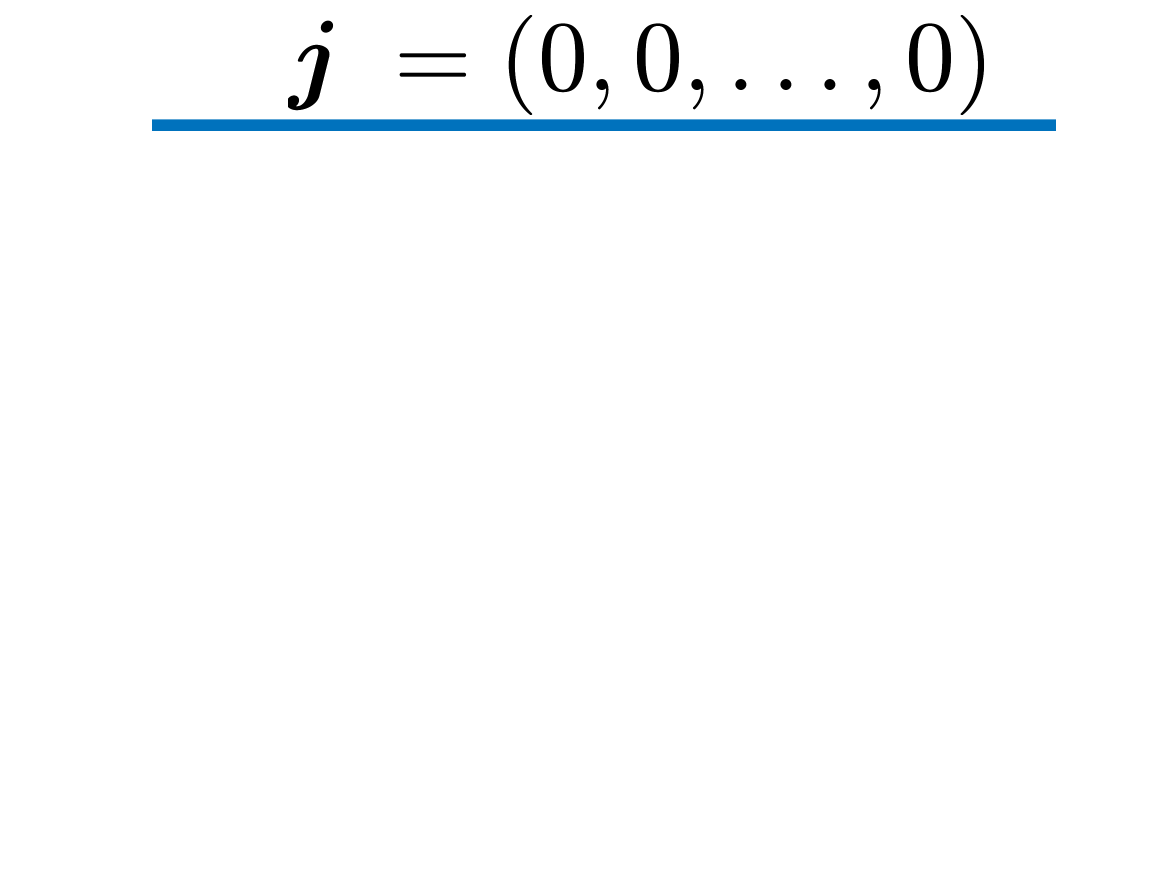
\includegraphics[width =0.18\textwidth]{ProgramsImages/Legendre_Degree_0.png}  &
		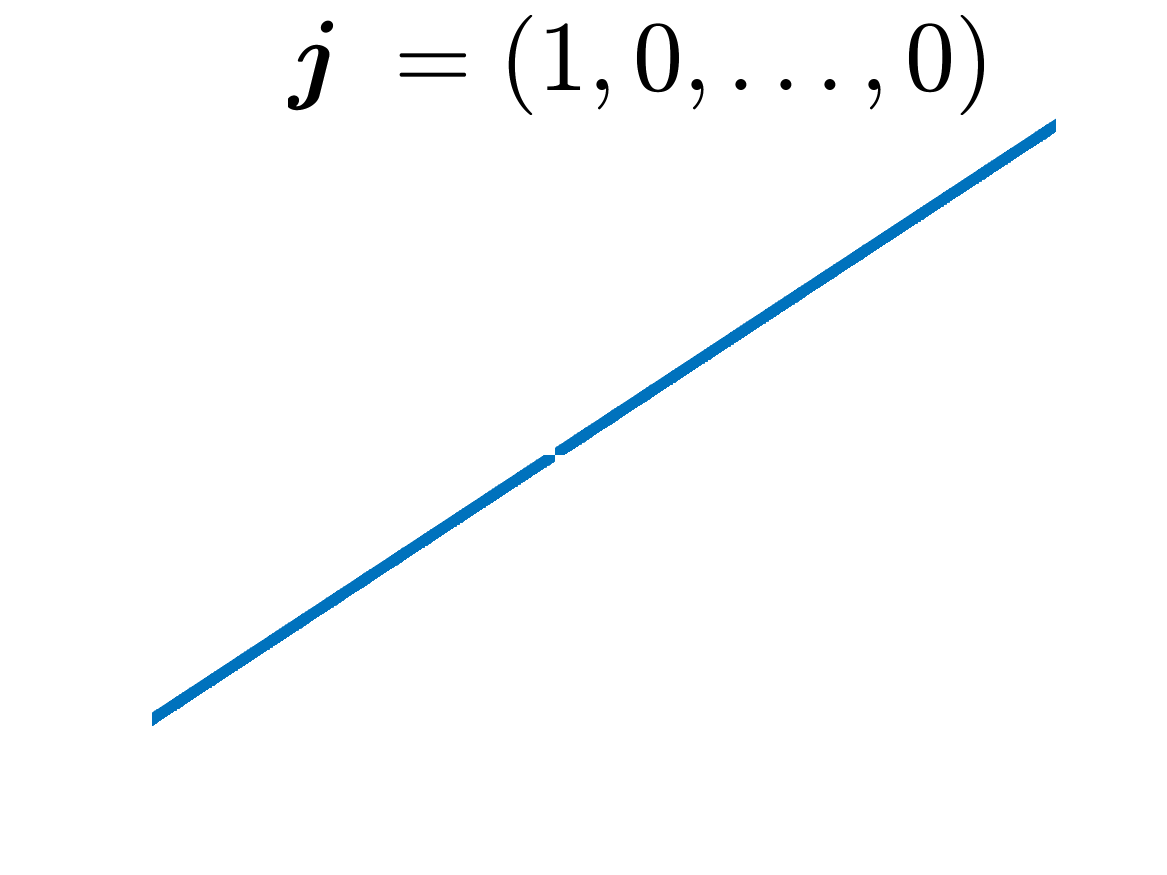
\includegraphics[width =0.18\textwidth]{ProgramsImages/Legendre_Degree_1.png}  &
		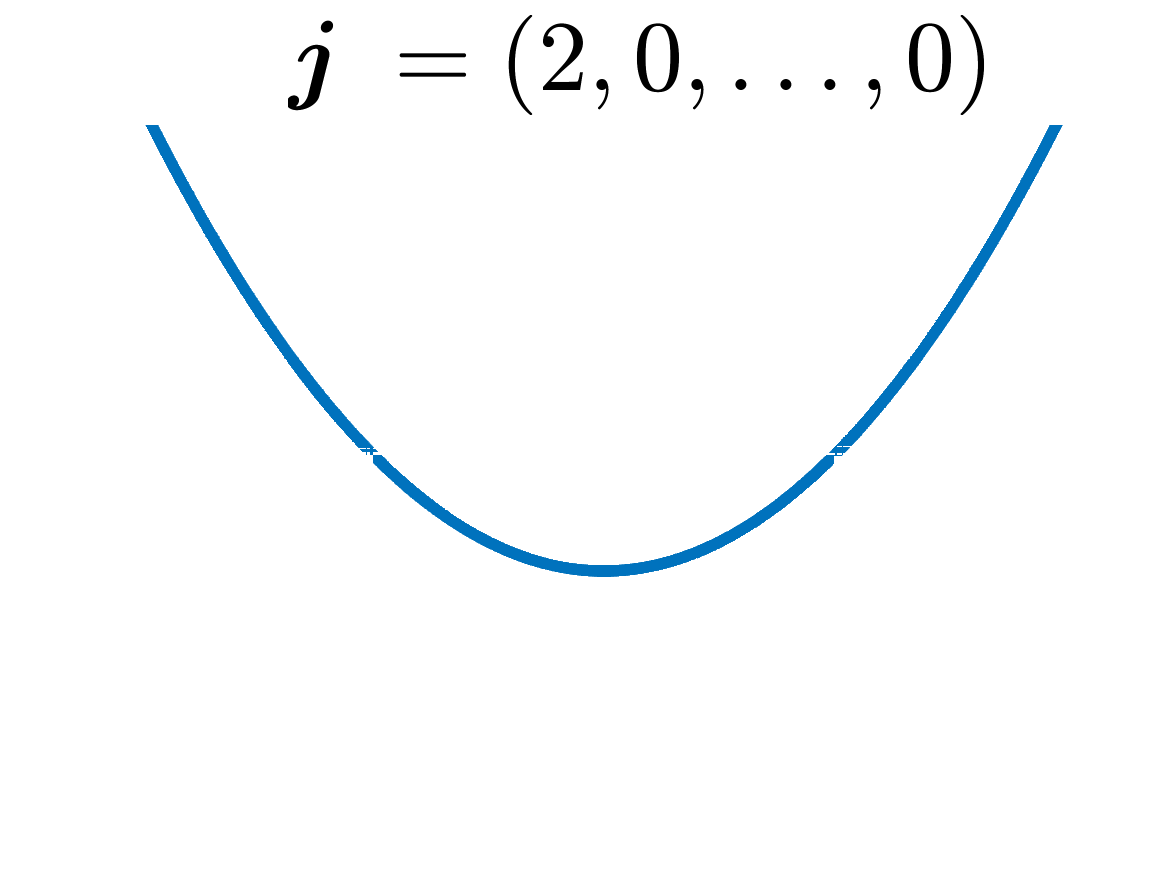
\includegraphics[width =0.18\textwidth]{ProgramsImages/Legendre_Degree_2.png}  &
		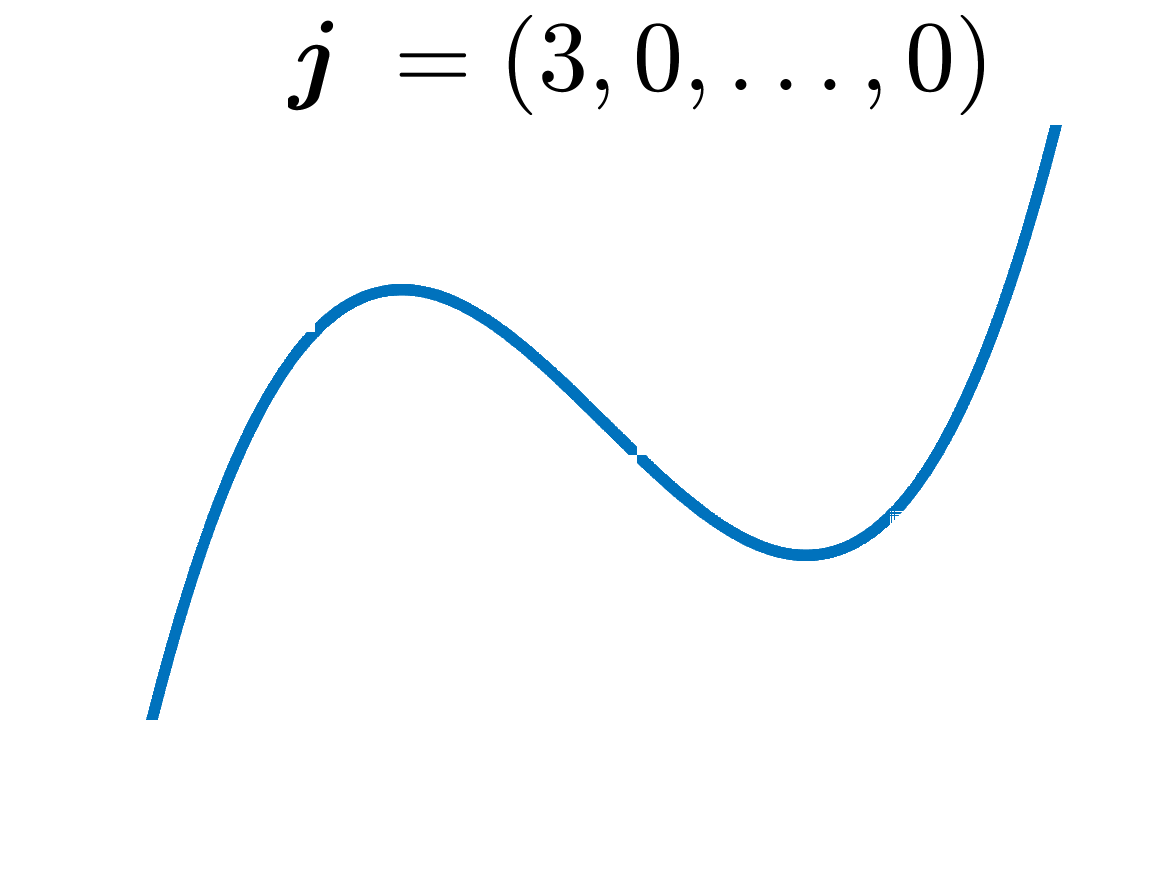
\includegraphics[width =0.18\textwidth]{ProgramsImages/Legendre_Degree_3.png}  &
		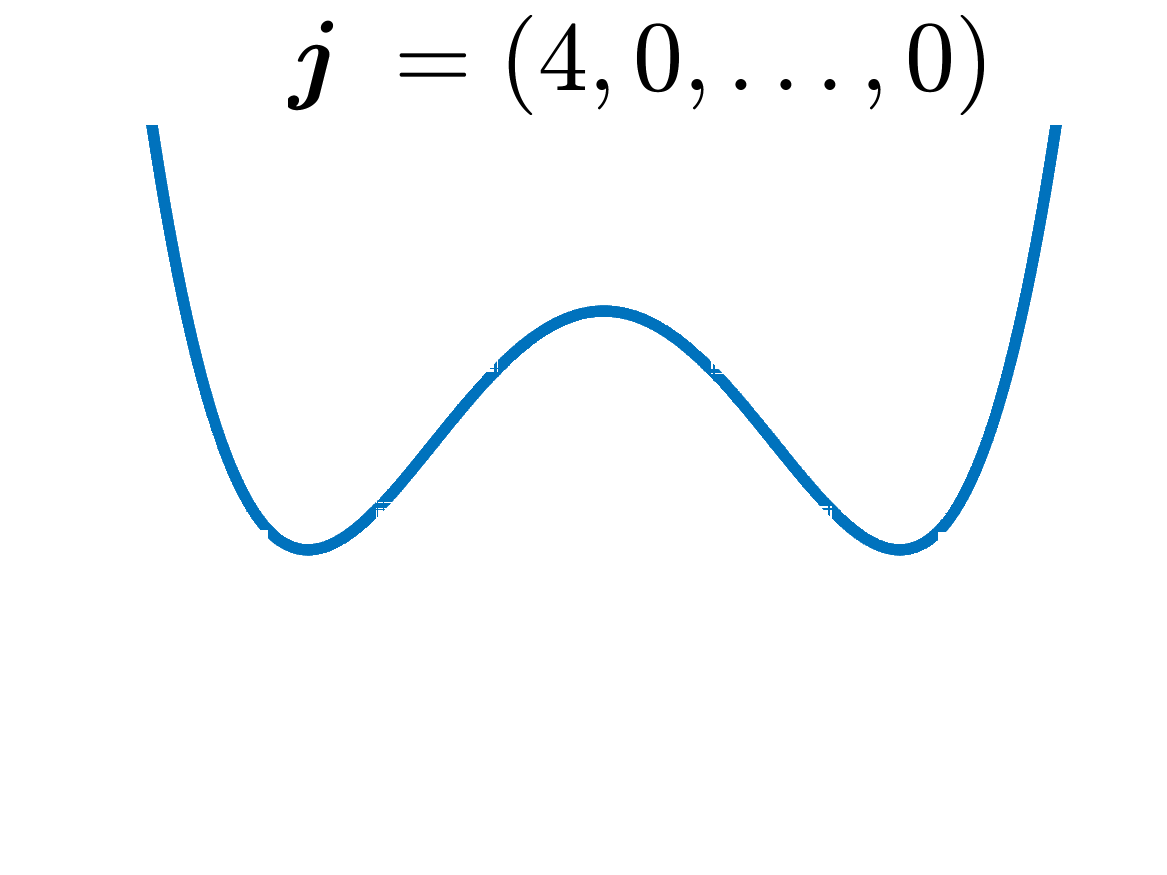
\includegraphics[width =0.18\textwidth]{ProgramsImages/Legendre_Degree_4.png} 
	\tabularnewline[-7ex]
	Legendre
	\tabularnewline
	\tabularnewline
		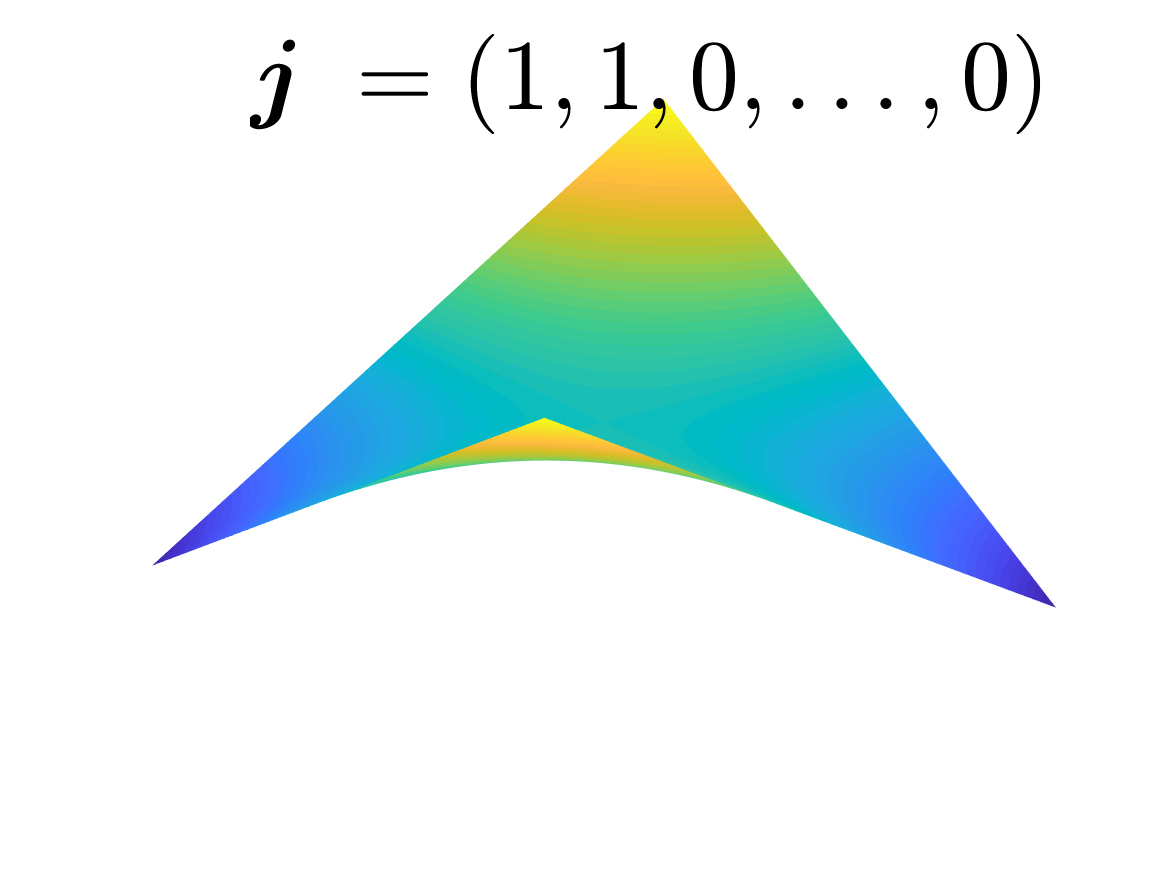
\includegraphics[width =0.18\textwidth]{ProgramsImages/Legendre_Degree_1_1.png}  &
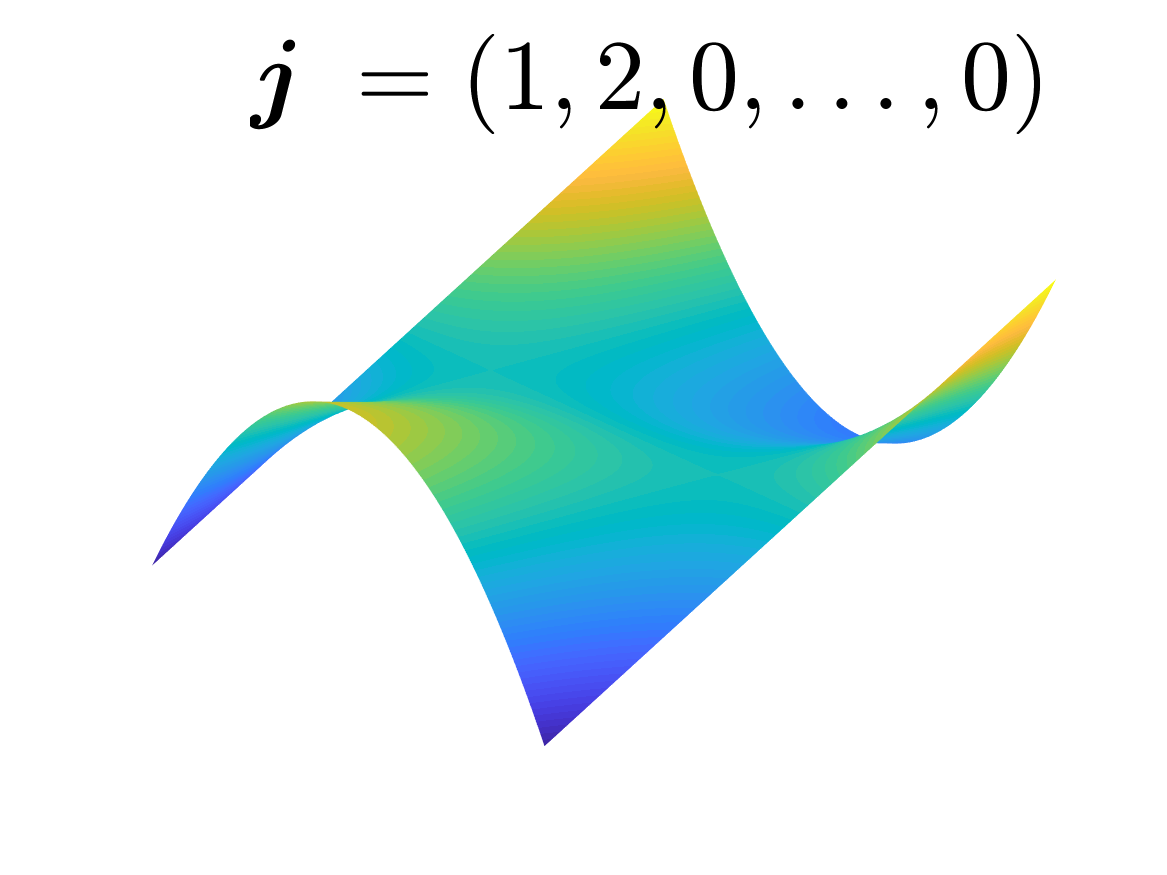
\includegraphics[width =0.18\textwidth]{ProgramsImages/Legendre_Degree_1_2.png}  &
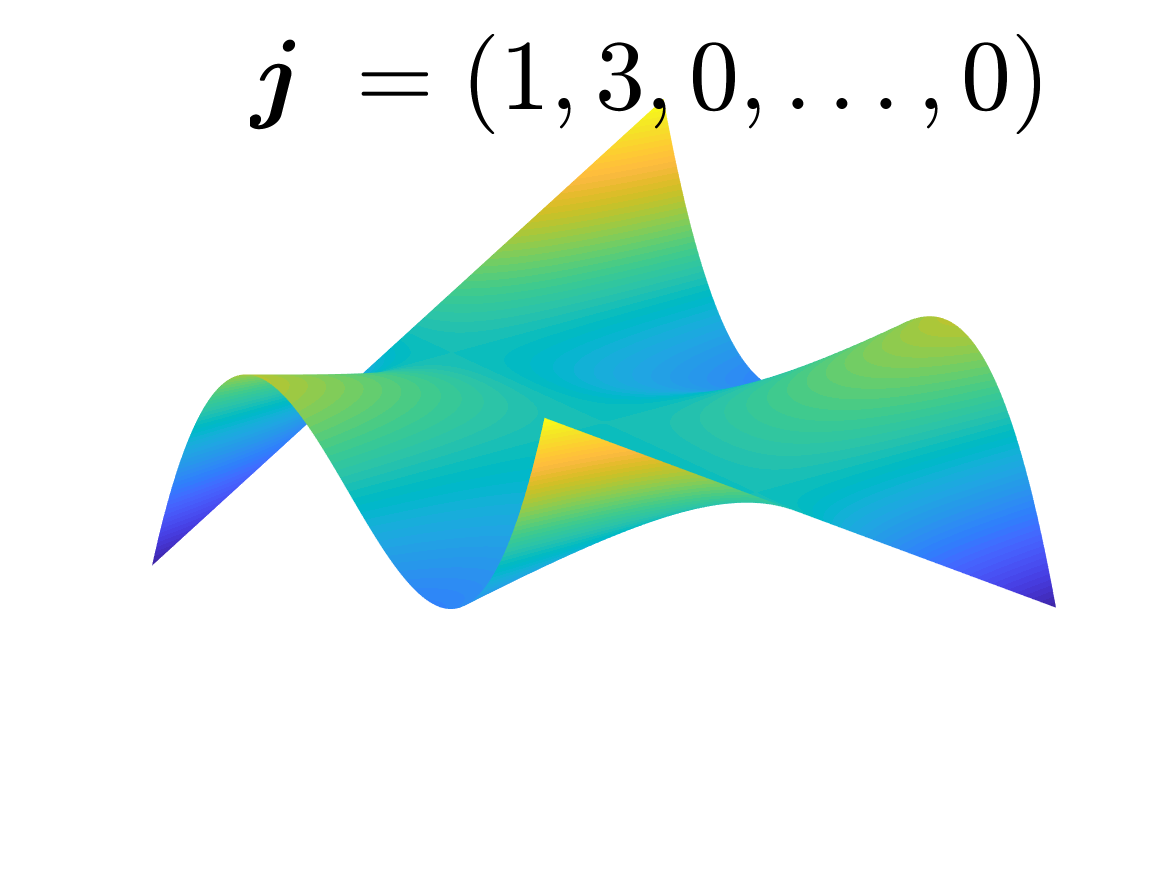
\includegraphics[width =0.18\textwidth]{ProgramsImages/Legendre_Degree_1_3.png}  &
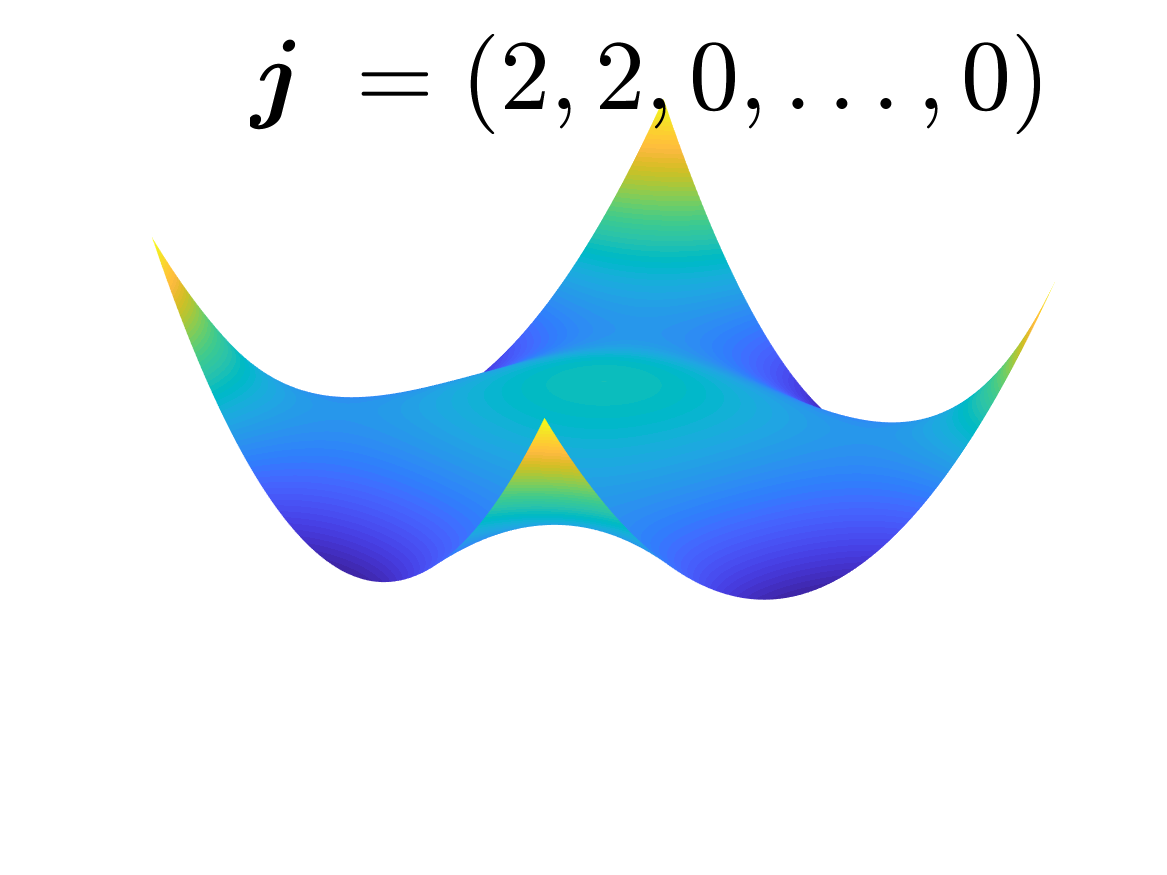
\includegraphics[width =0.18\textwidth]{ProgramsImages/Legendre_Degree_2_2.png}  &
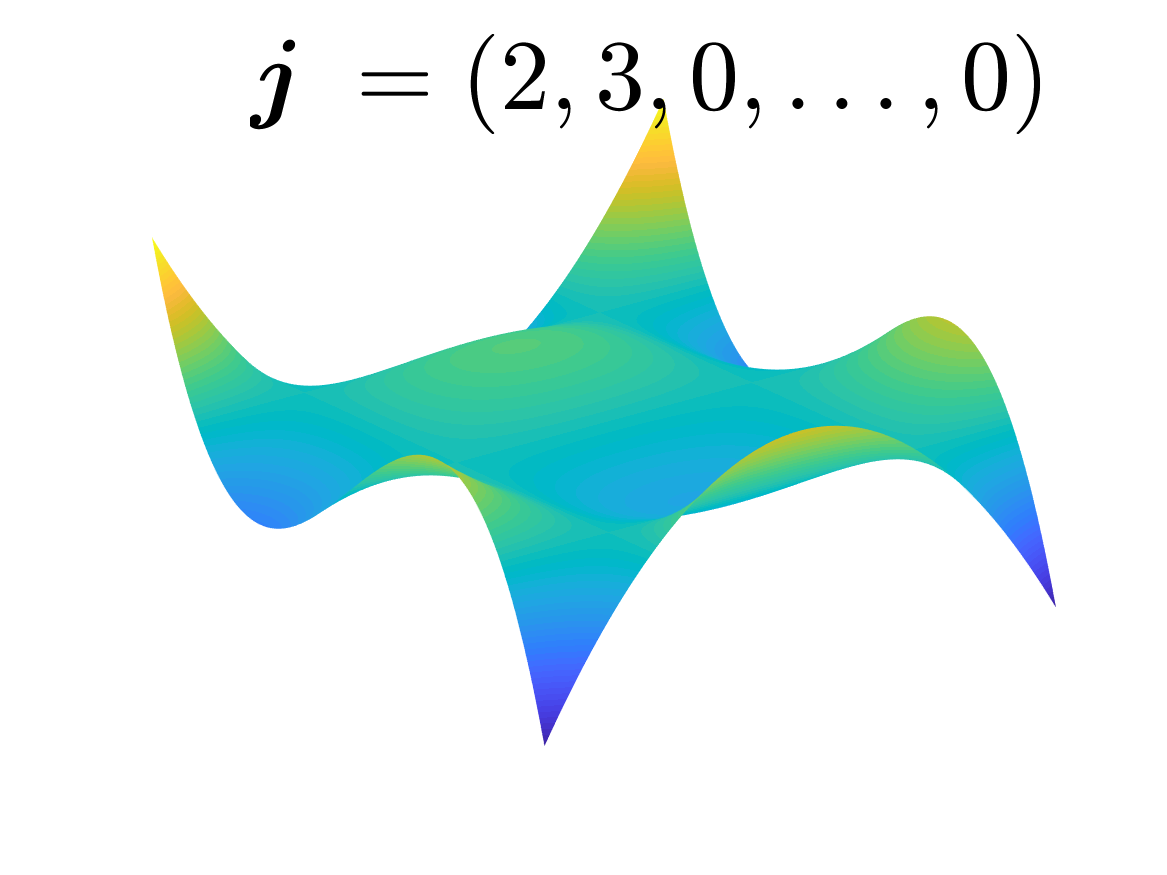
\includegraphics[width =0.18\textwidth]{ProgramsImages/Legendre_Degree_2_3.png} 
\tabularnewline[0ex]
		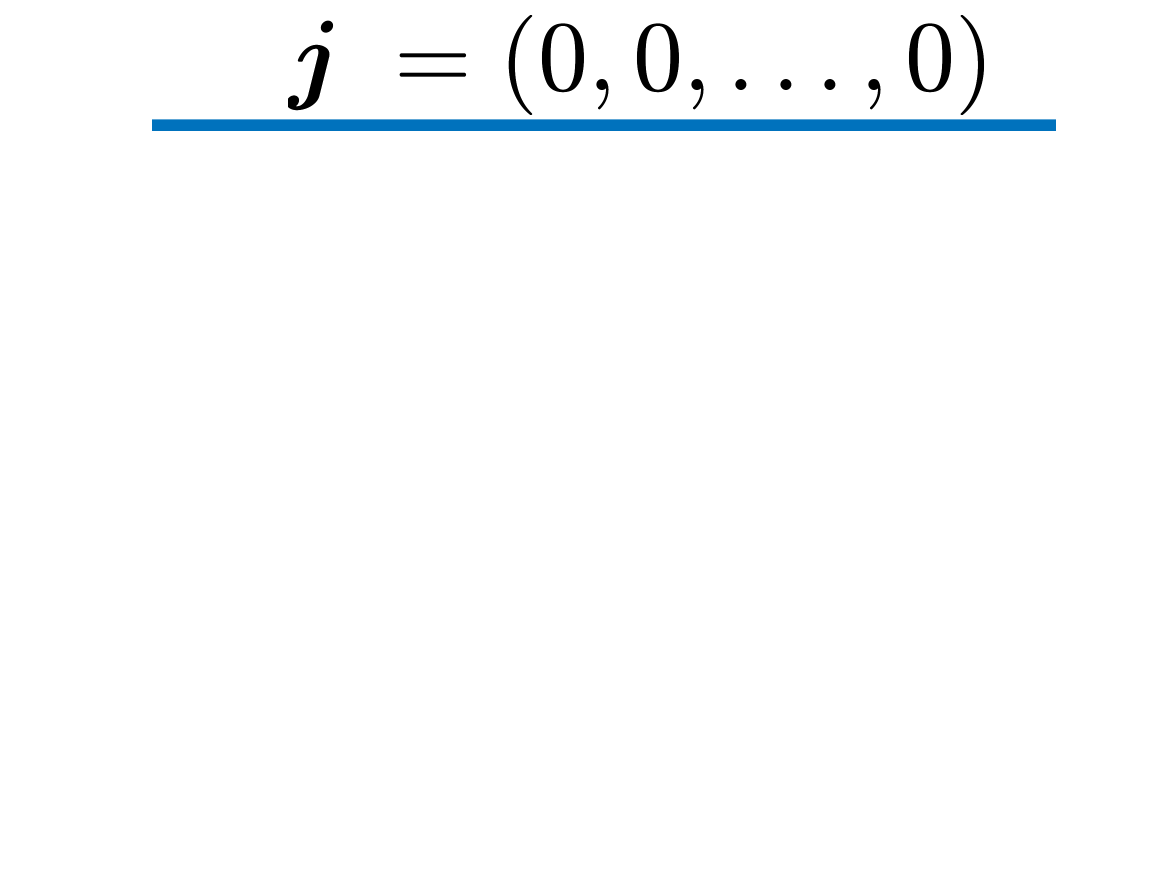
\includegraphics[width =0.18\textwidth]{ProgramsImages/Chebyshev_Degree_0.png}  &
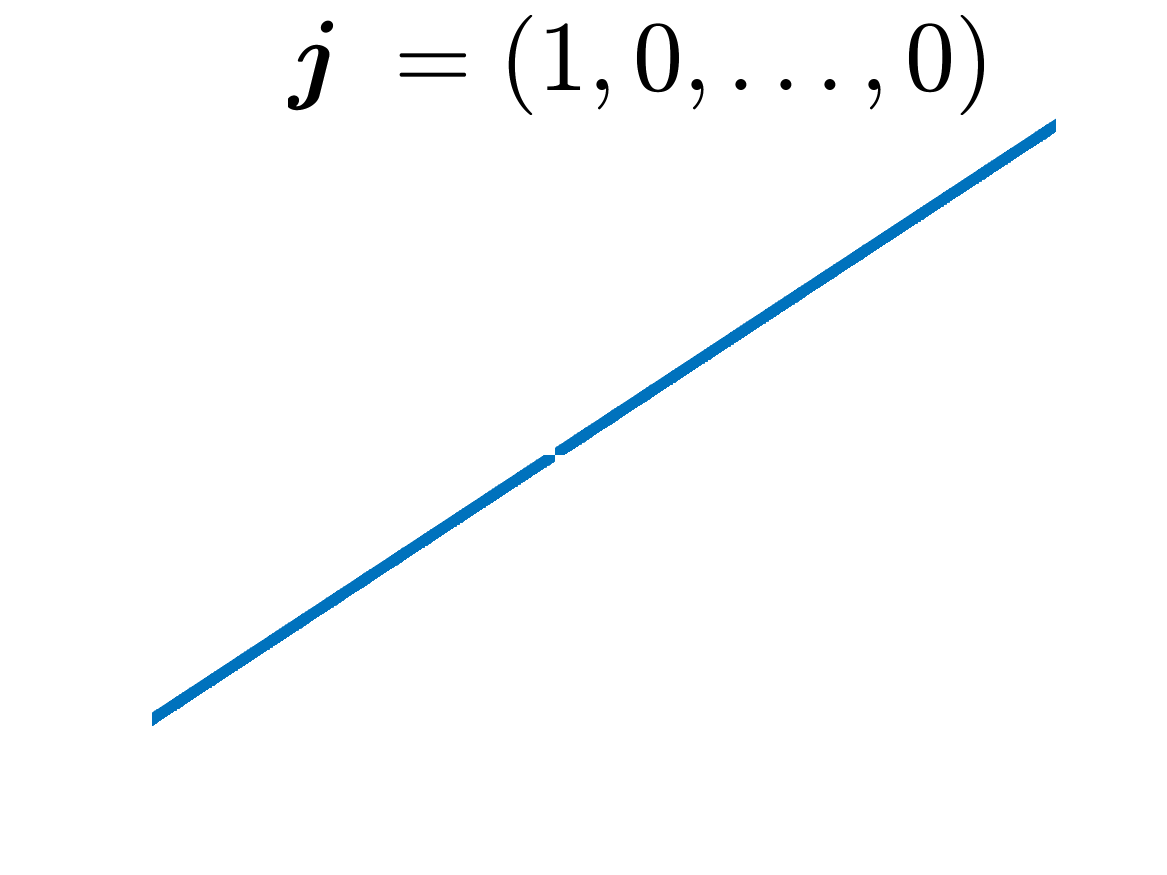
\includegraphics[width =0.18\textwidth]{ProgramsImages/Chebyshev_Degree_1.png}  &
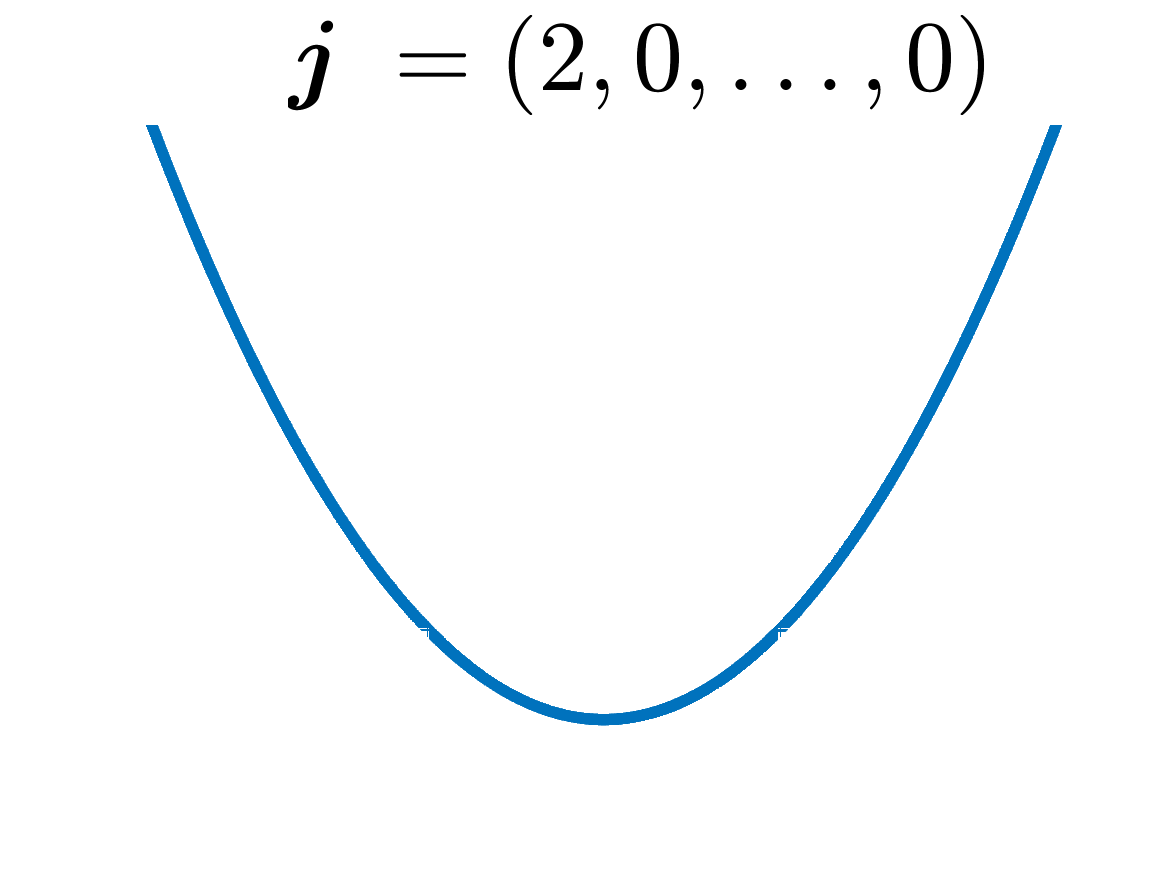
\includegraphics[width =0.18\textwidth]{ProgramsImages/Chebyshev_Degree_2.png}  &
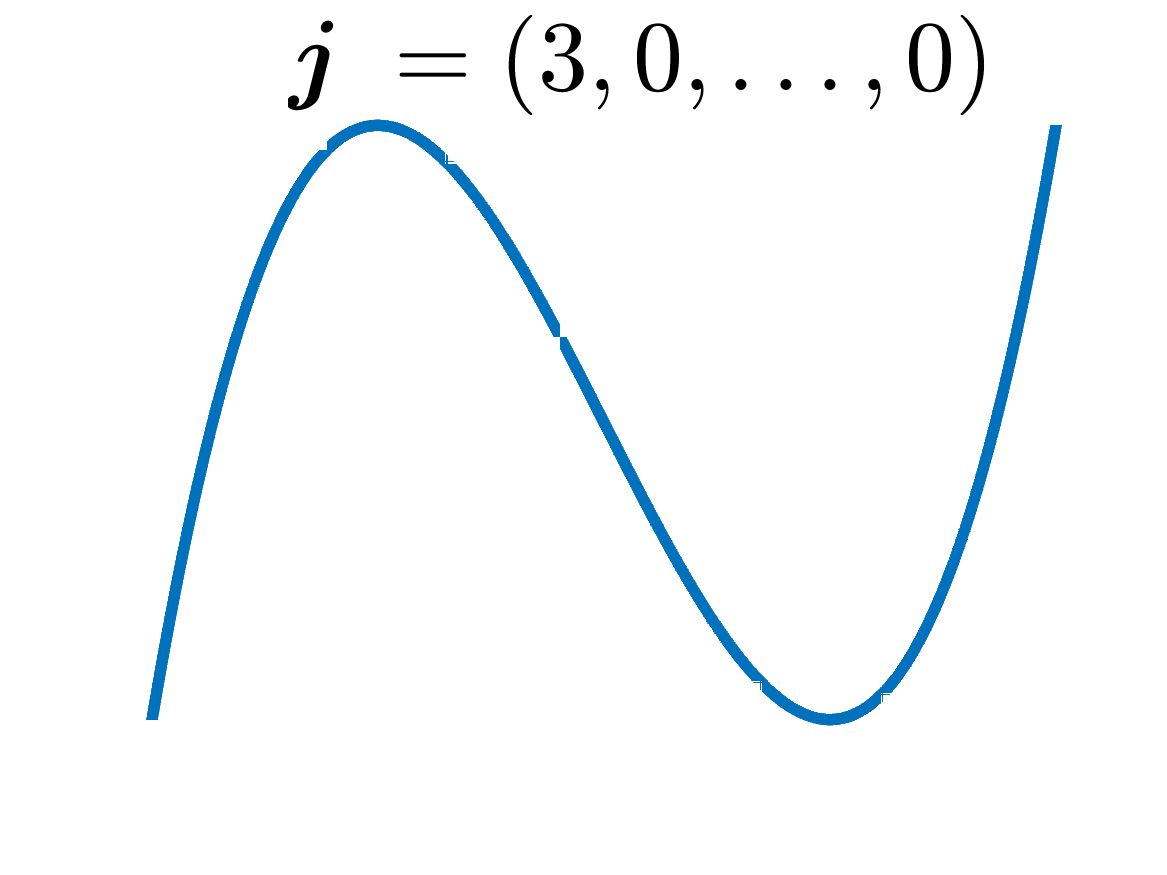
\includegraphics[width =0.18\textwidth]{ProgramsImages/Chebyshev_Degree_3.png}  &
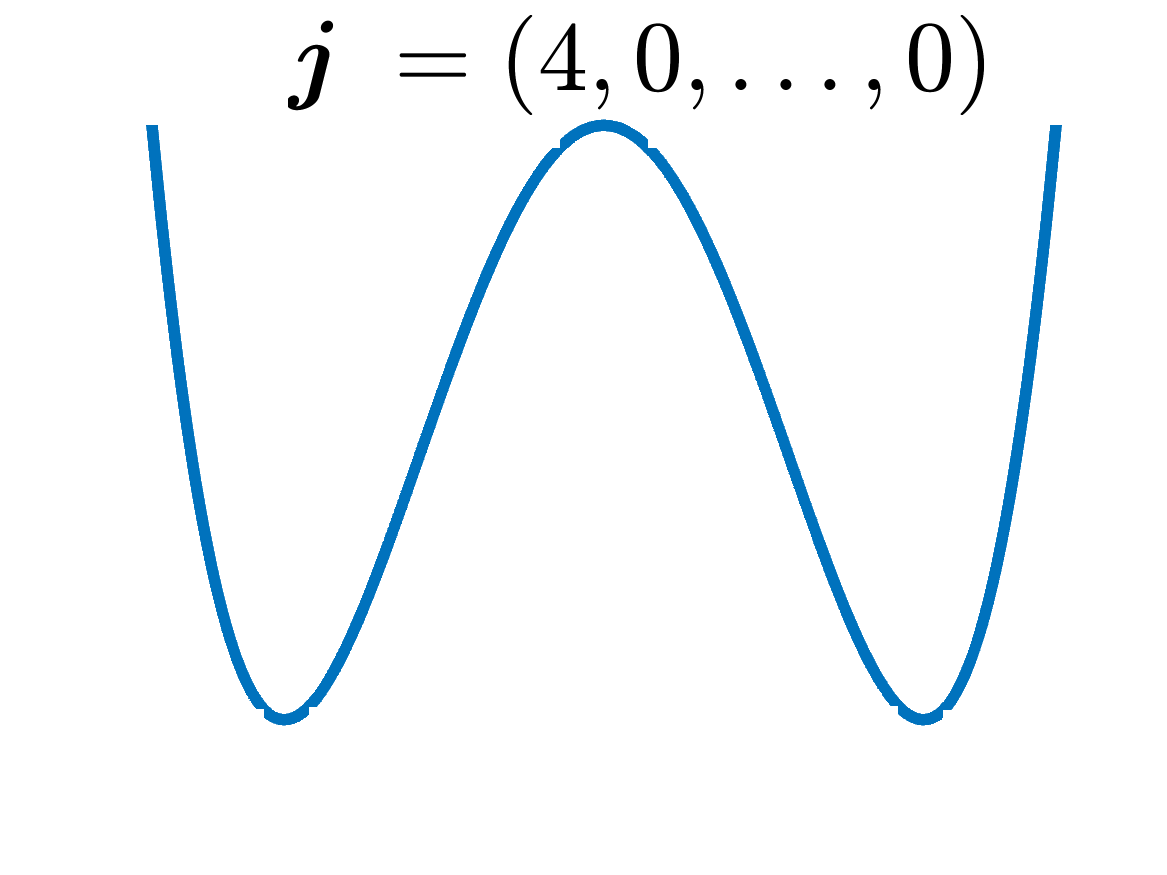
\includegraphics[width =0.18\textwidth]{ProgramsImages/Chebyshev_Degree_4.png} 
\tabularnewline[-7ex]
Chebyshev \tabularnewline
\tabularnewline
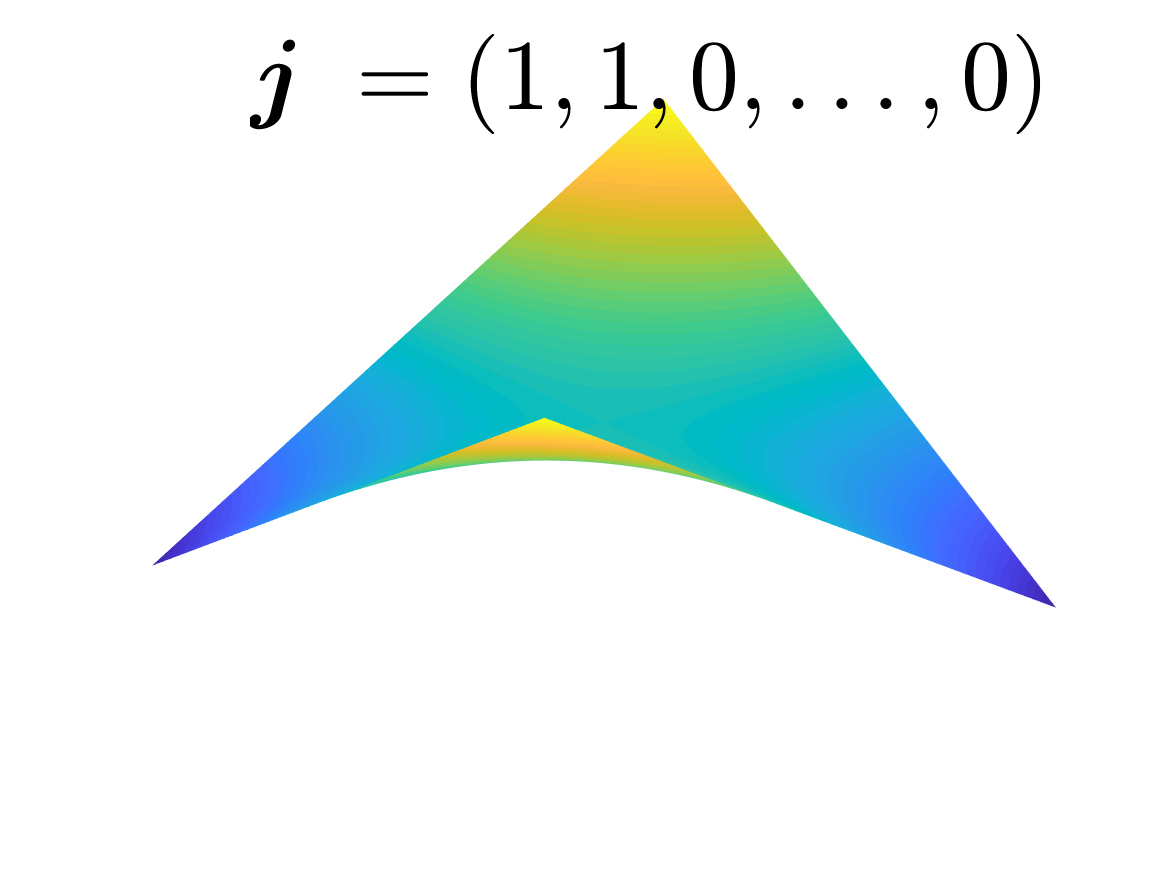
\includegraphics[width =0.18\textwidth]{ProgramsImages/Chebyshev_Degree_1_1.png}  &
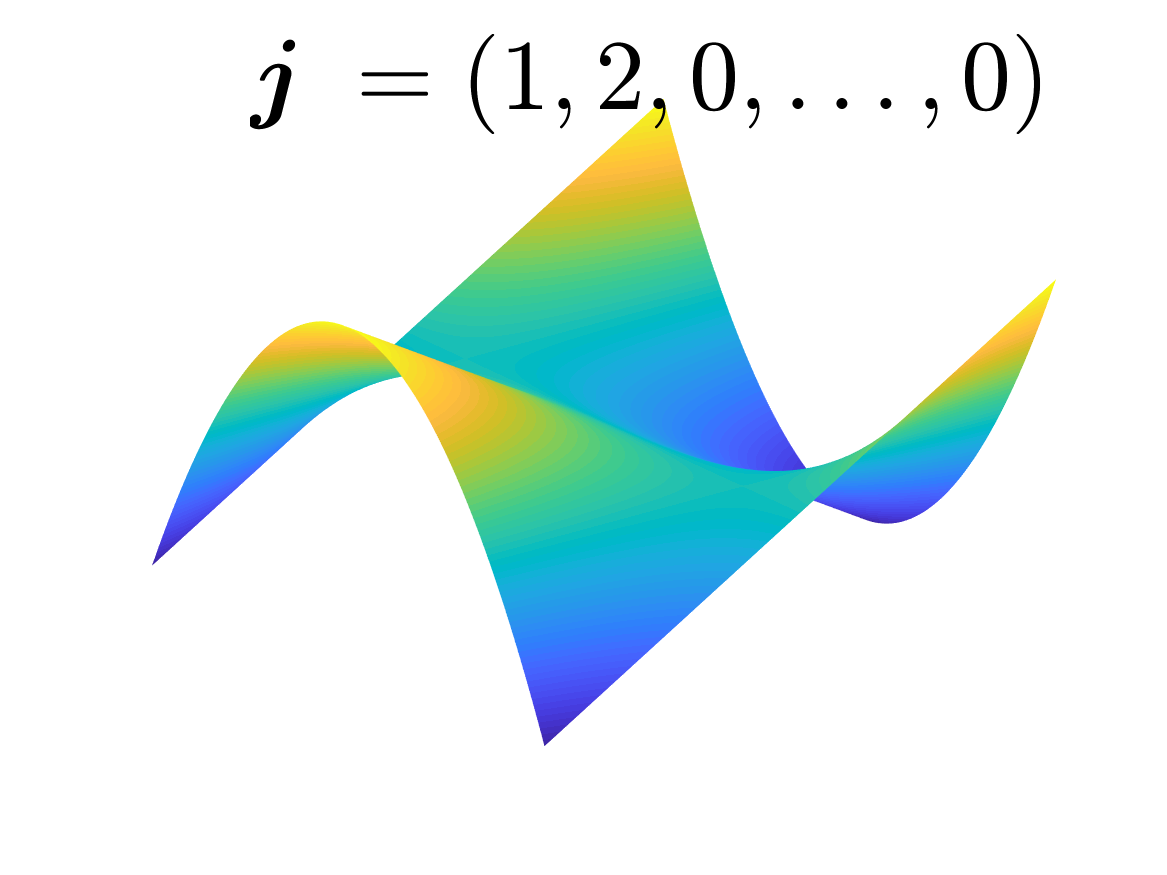
\includegraphics[width =0.18\textwidth]{ProgramsImages/Chebyshev_Degree_1_2.png}  &
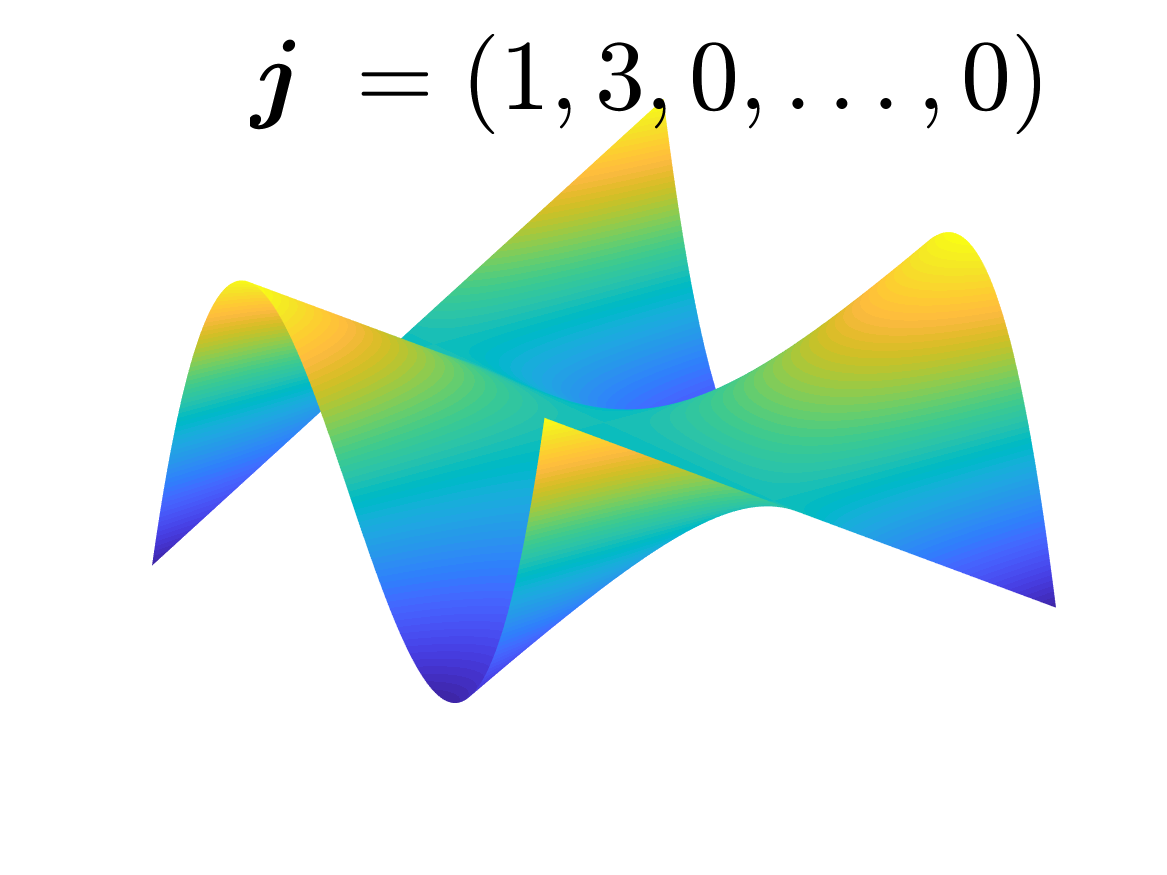
\includegraphics[width =0.18\textwidth]{ProgramsImages/Chebyshev_Degree_1_3.png}  &
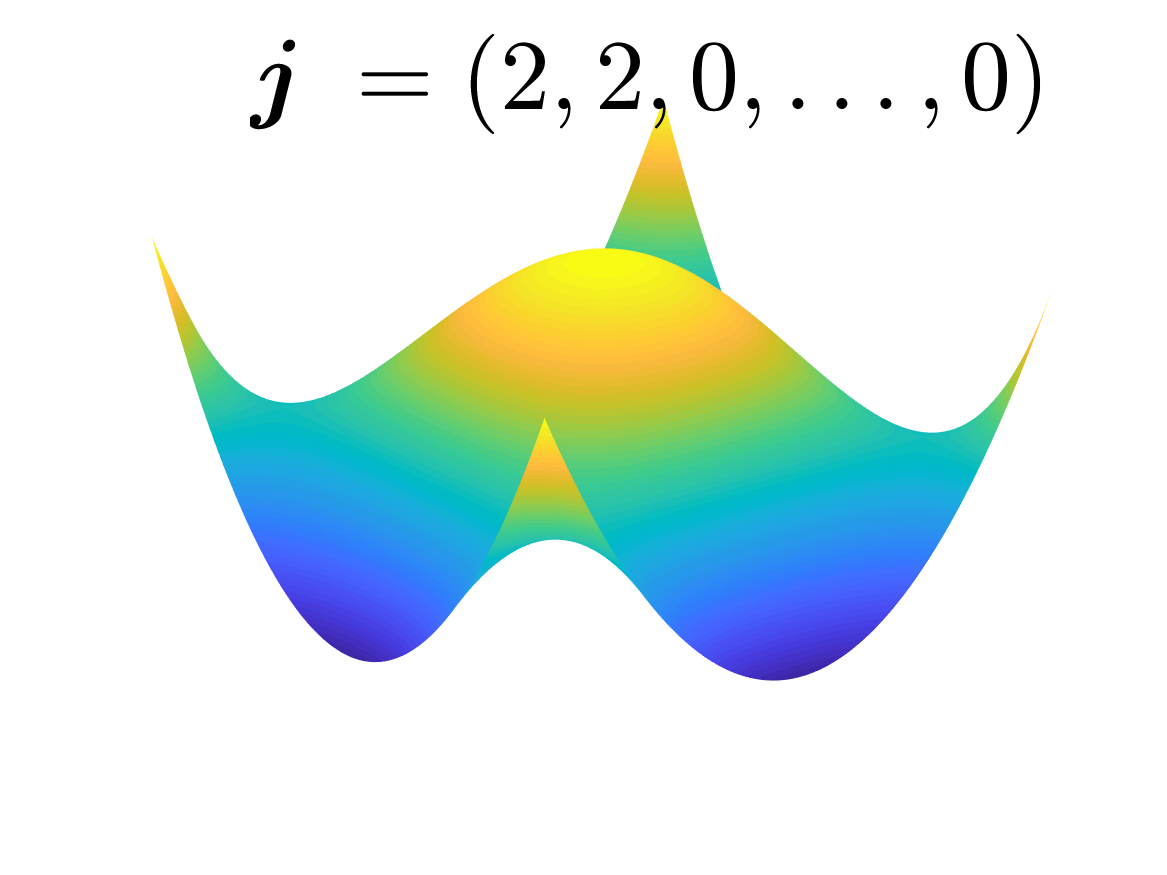
\includegraphics[width =0.18\textwidth]{ProgramsImages/Chebyshev_Degree_2_2.png}  &
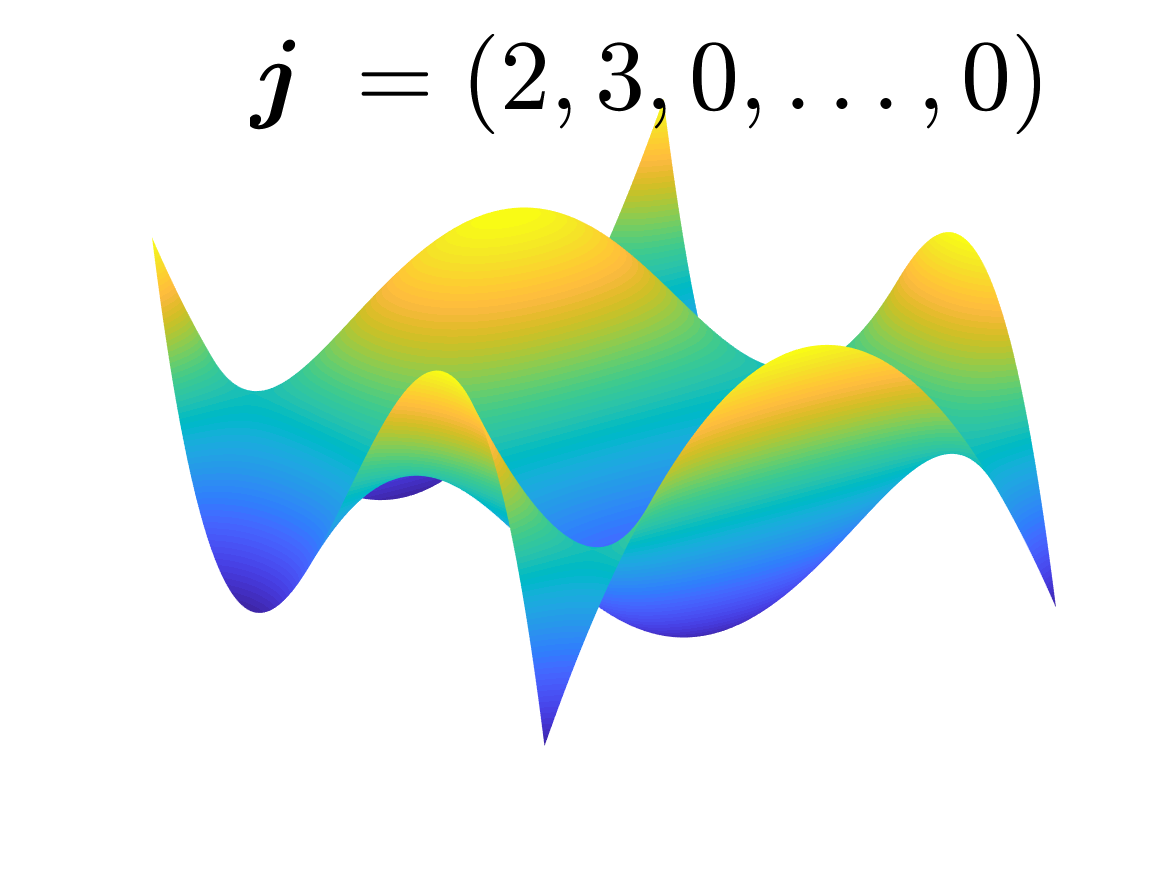
\includegraphics[width =0.18\textwidth]{ProgramsImages/Chebyshev_Degree_2_3.png} 
	\end{tabular}
\end{frame}

\section{Integration}

\begin{frame}
\frametitle{Complex Exponential and Walsh Bases}
\vspace{-3ex}
	\begin{tabular}{>{\centering}m{0.18\textwidth}>{\centering}m{0.18\textwidth}>{\centering}m{0.18\textwidth}>{\centering}m{0.18\textwidth}>{\centering}m{0.18\textwidth}}
		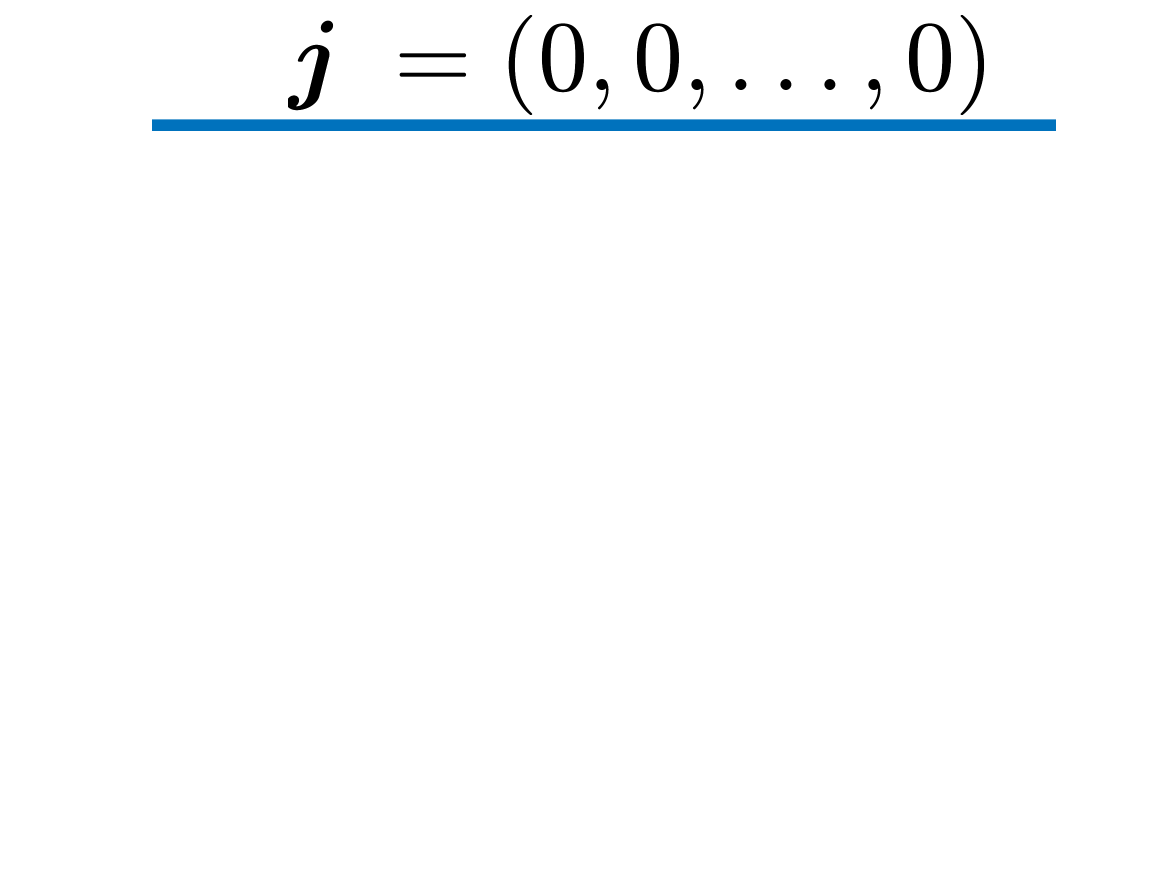
\includegraphics[width =0.18\textwidth]{ProgramsImages/CosineSine_Degree_0.png}  &
		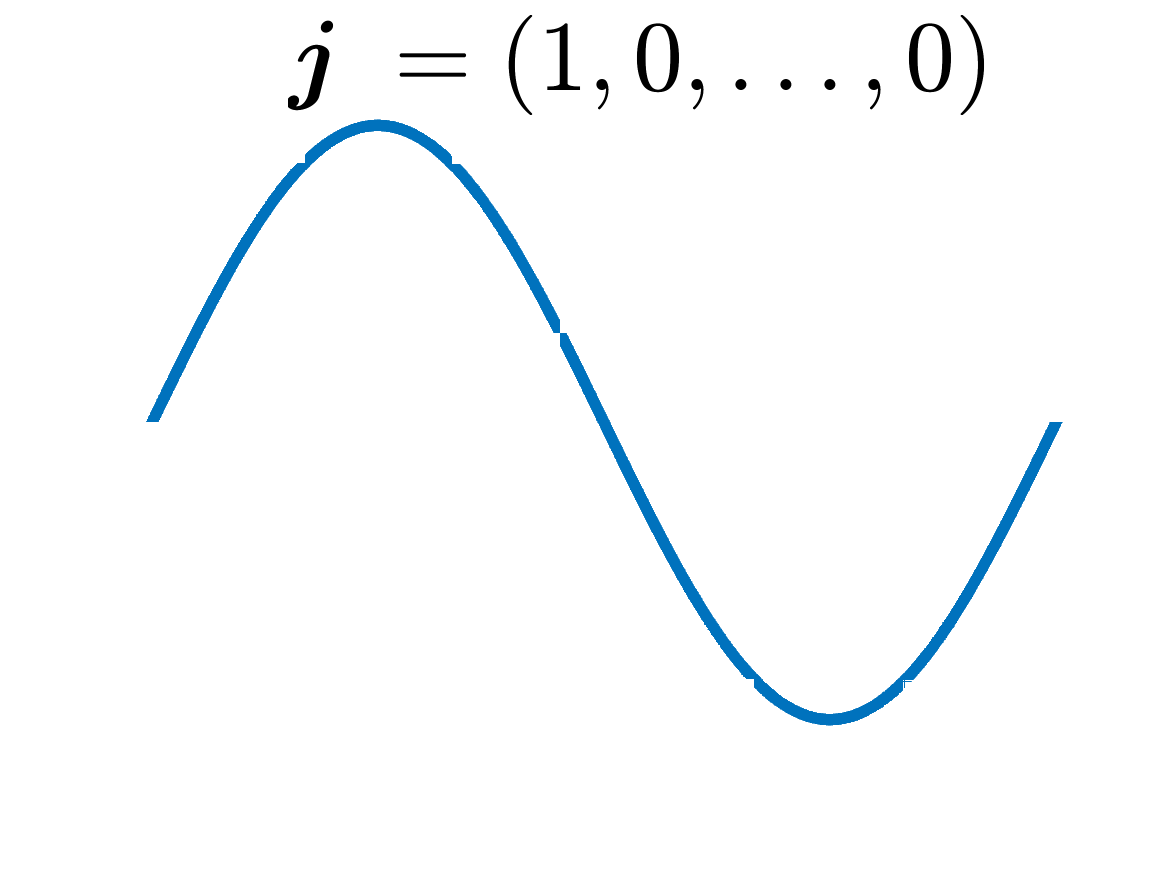
\includegraphics[width =0.18\textwidth]{ProgramsImages/CosineSine_Degree_1.png}  &
		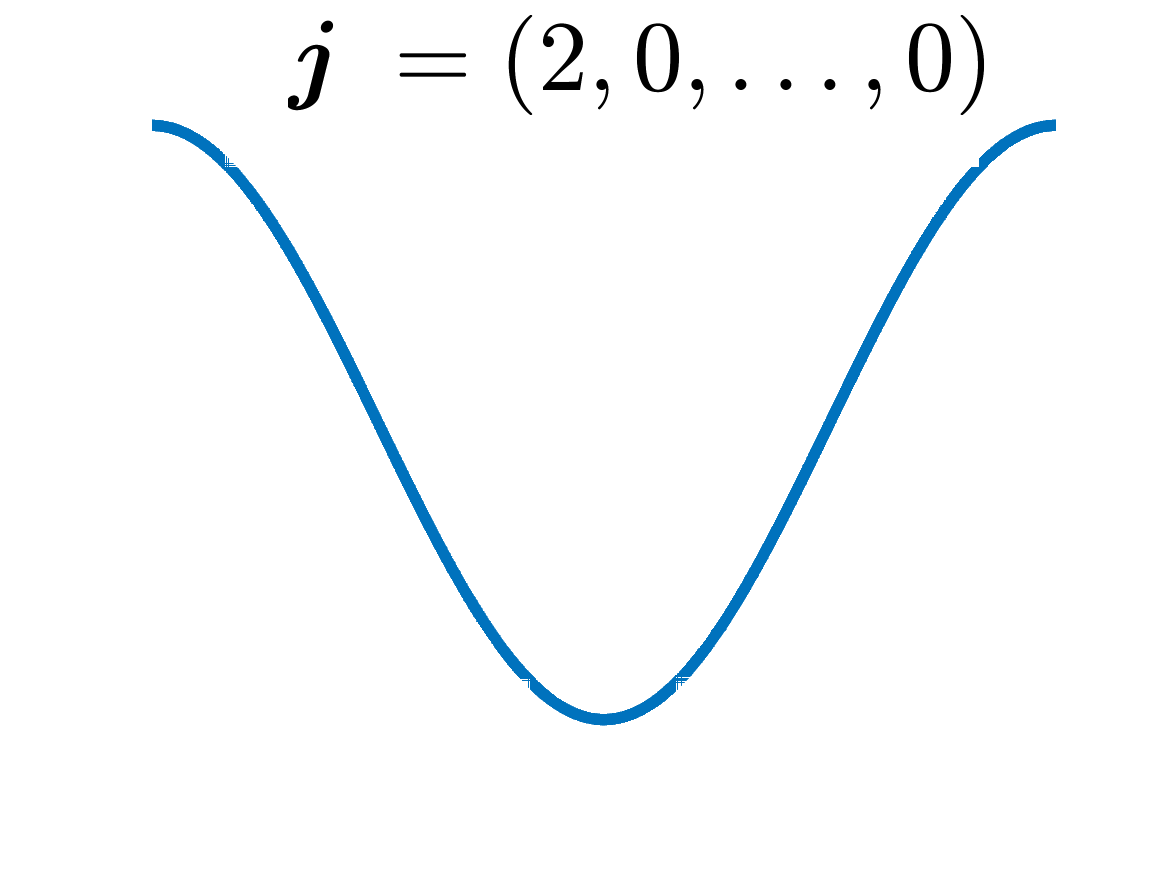
\includegraphics[width =0.18\textwidth]{ProgramsImages/CosineSine_Degree_2.png}  &
		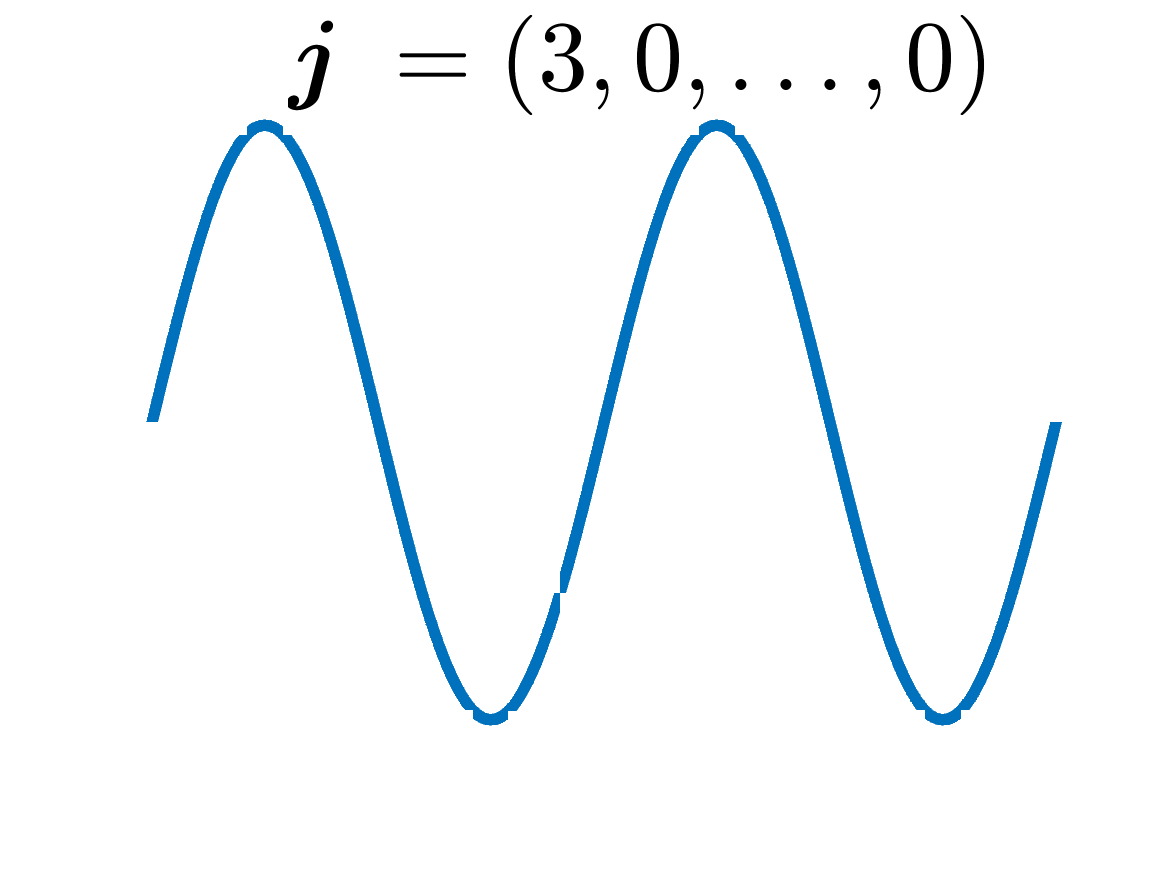
\includegraphics[width =0.18\textwidth]{ProgramsImages/CosineSine_Degree_3.png}  &
		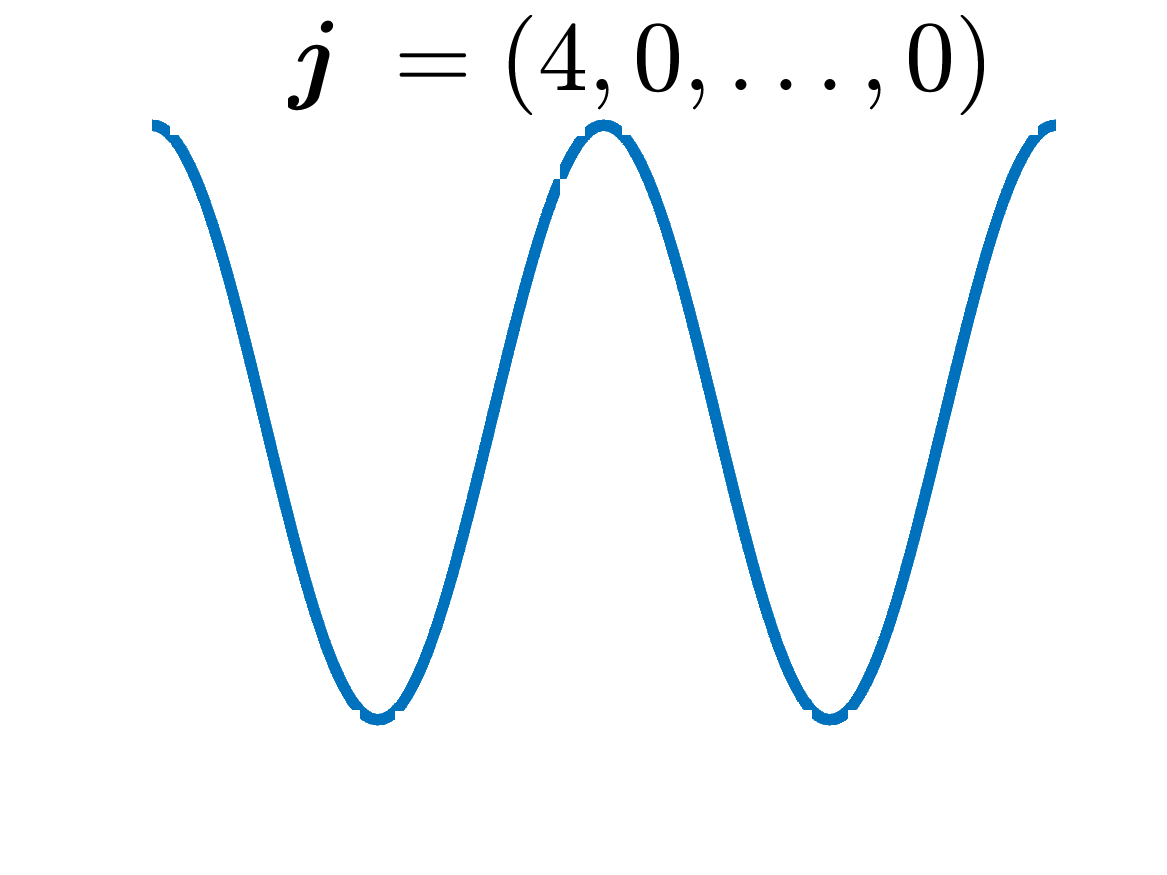
\includegraphics[width =0.18\textwidth]{ProgramsImages/CosineSine_Degree_4.png} 
	\tabularnewline[-7ex]
	Cosine \& Sine
	\tabularnewline
	\tabularnewline
		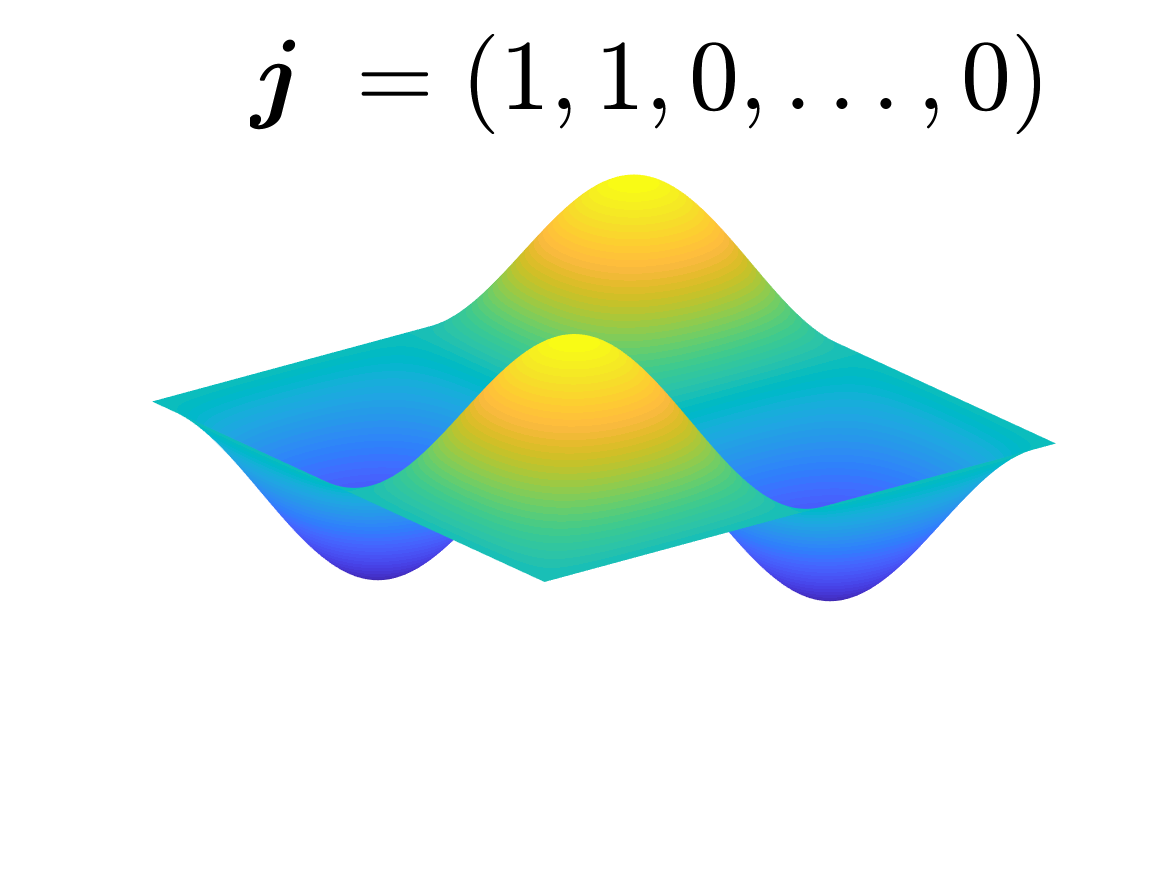
\includegraphics[width =0.18\textwidth]{ProgramsImages/CosineSine_Degree_1_1.png}  &
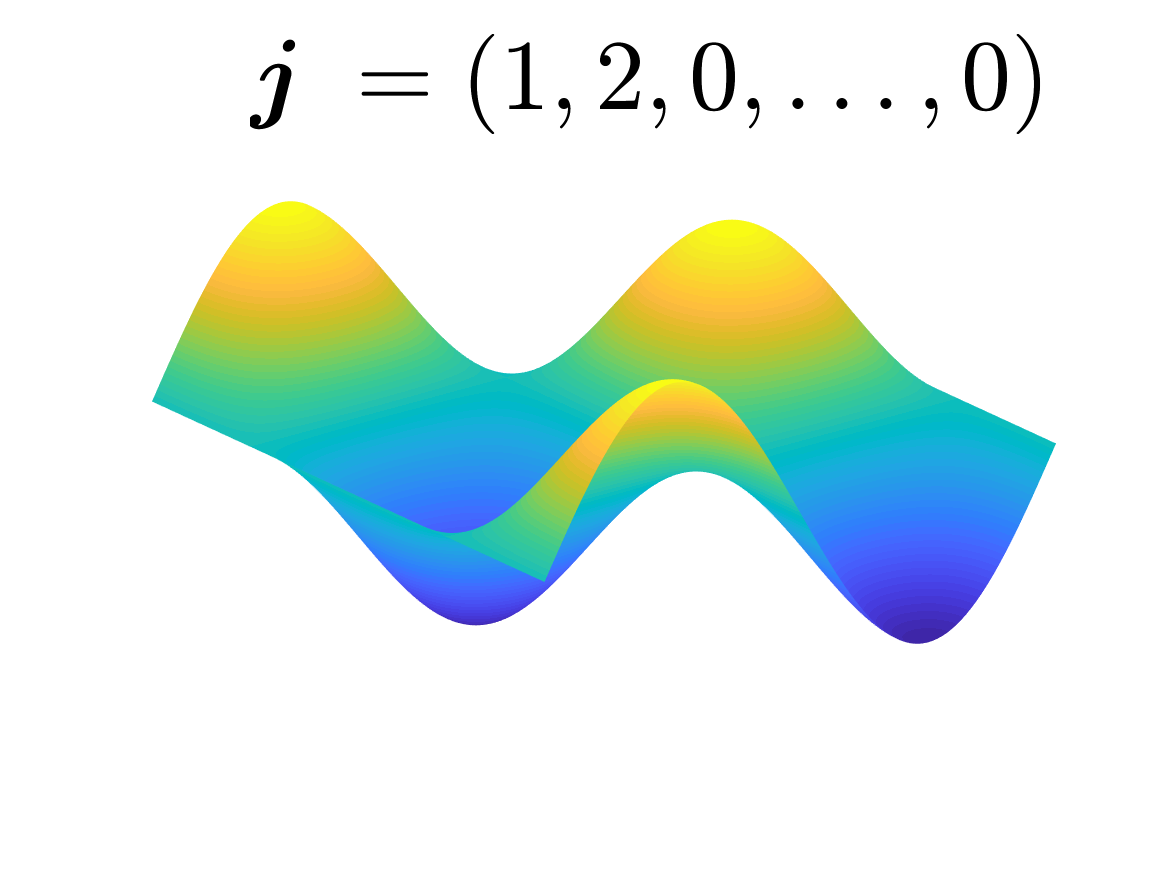
\includegraphics[width =0.18\textwidth]{ProgramsImages/CosineSine_Degree_1_2.png}  &
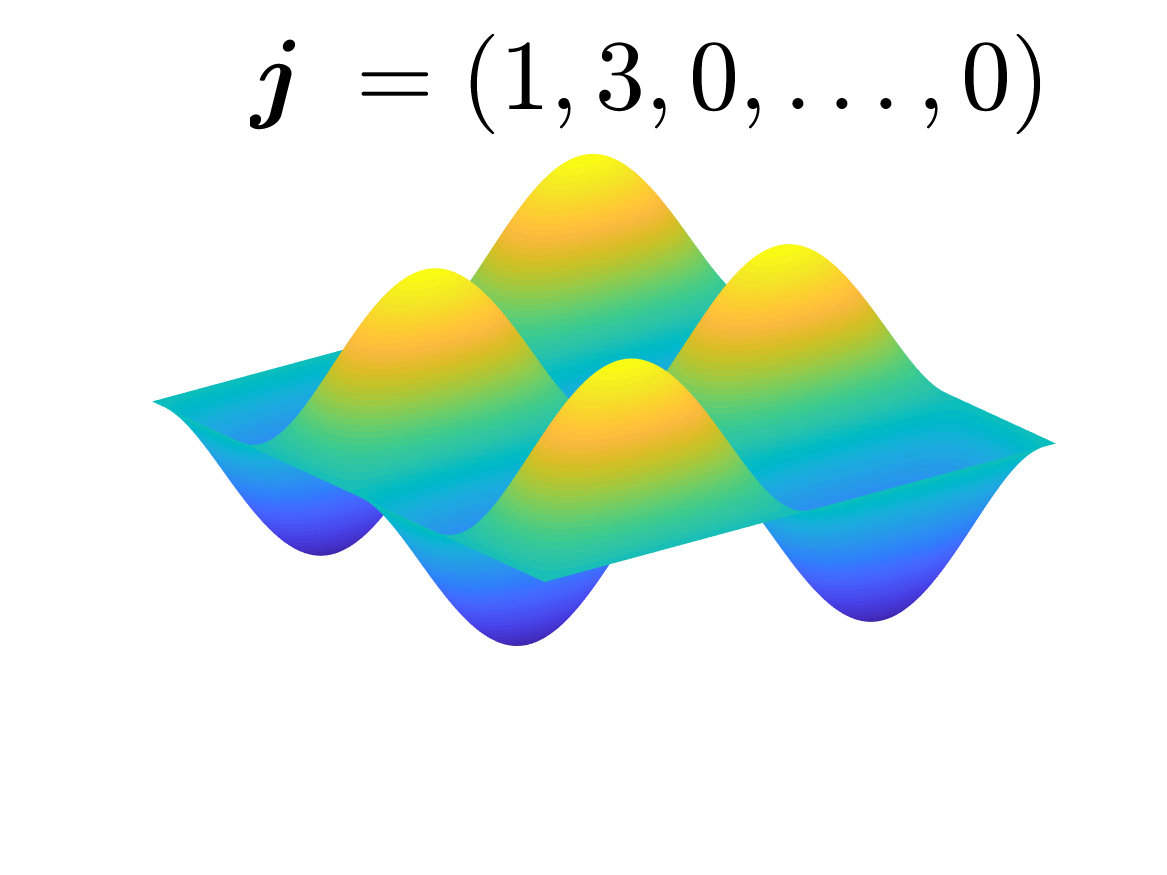
\includegraphics[width =0.18\textwidth]{ProgramsImages/CosineSine_Degree_1_3.png}  &
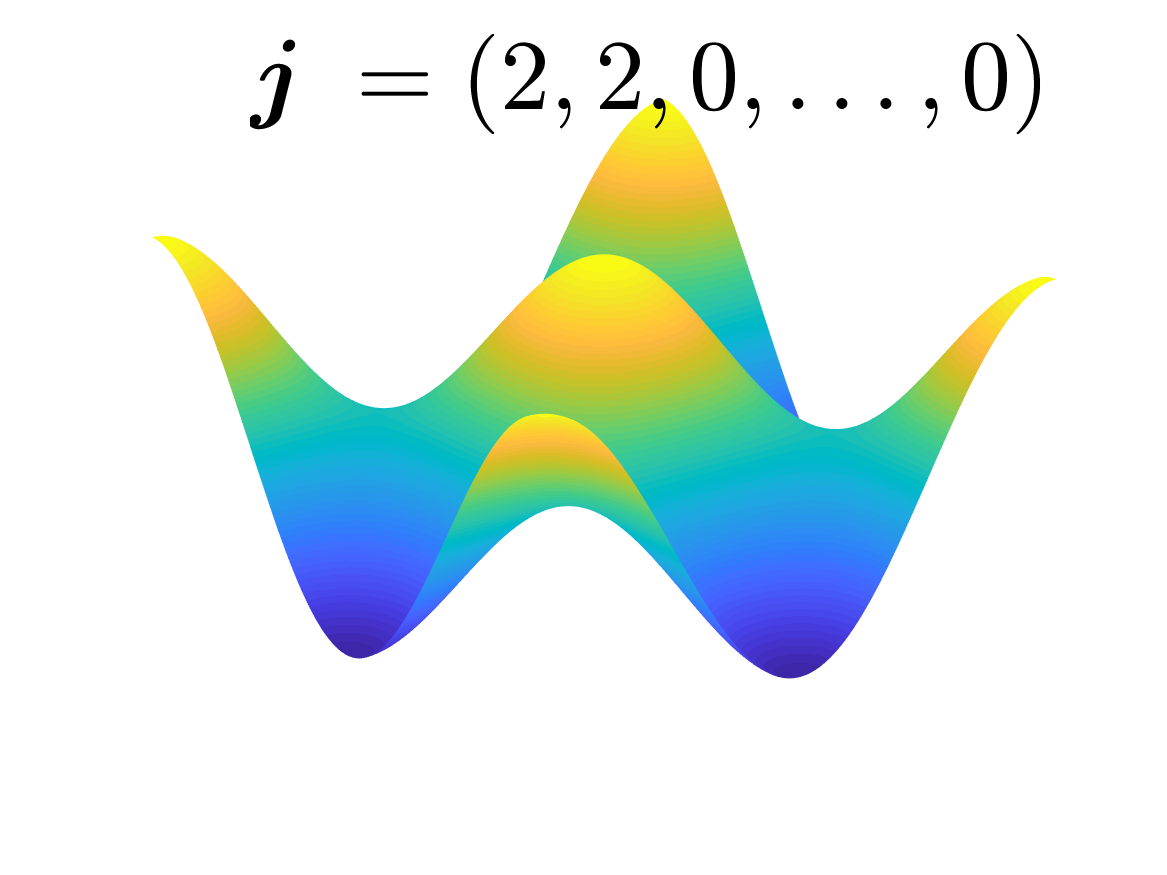
\includegraphics[width =0.18\textwidth]{ProgramsImages/CosineSine_Degree_2_2.png}  &
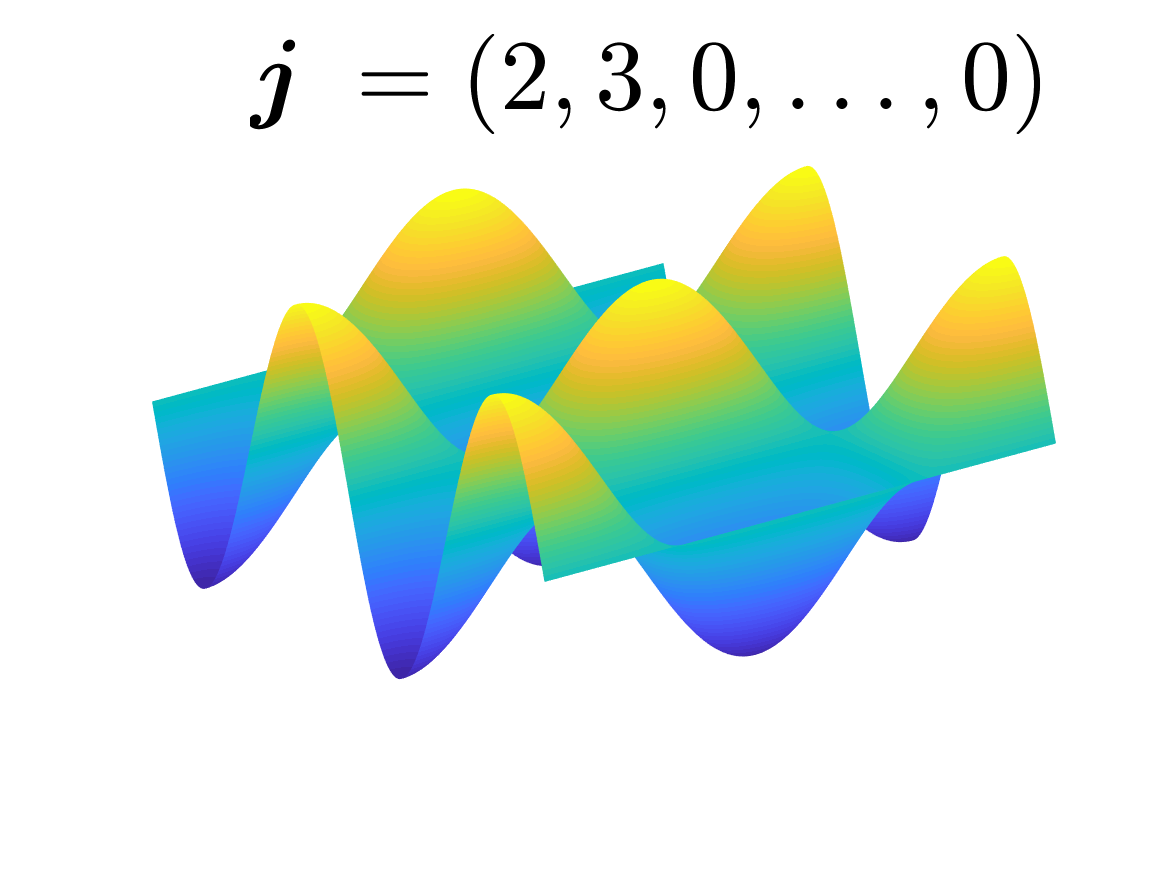
\includegraphics[width =0.18\textwidth]{ProgramsImages/CosineSine_Degree_2_3.png} 
\tabularnewline[0ex]
		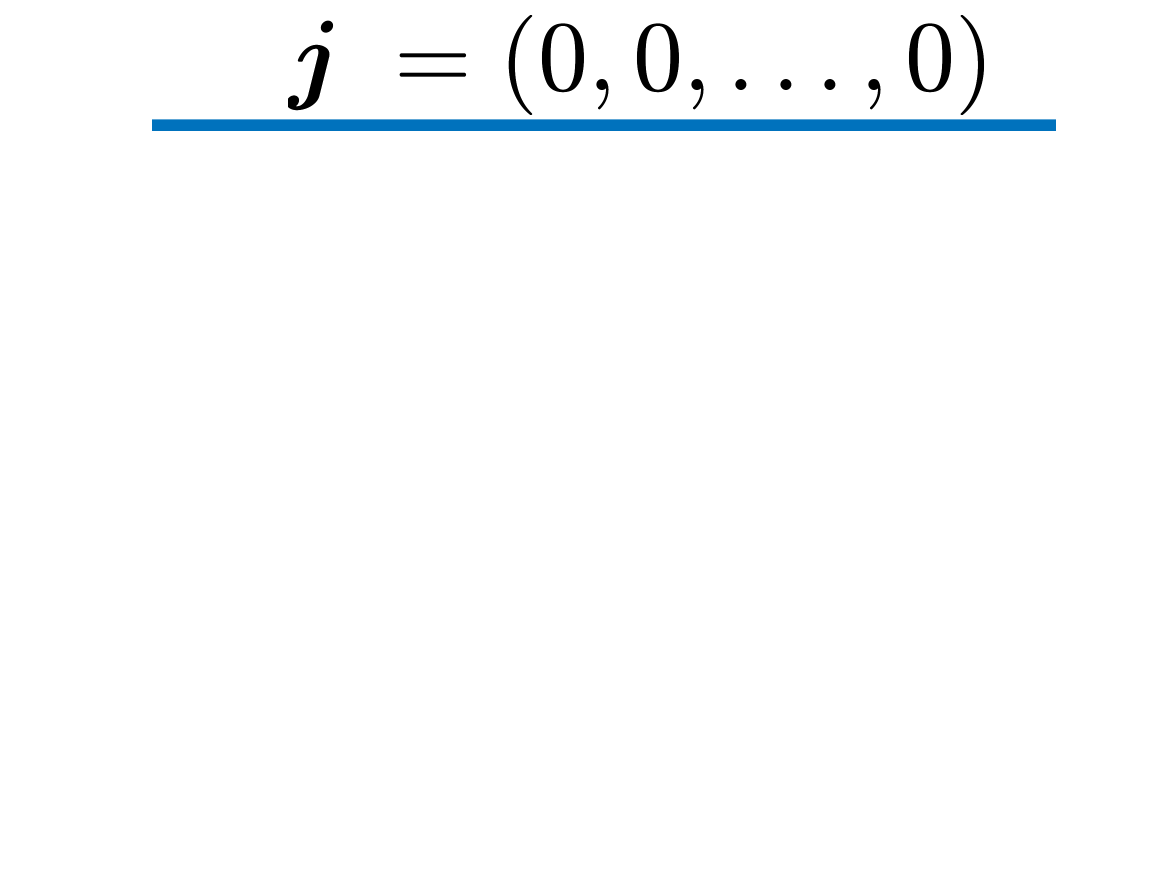
\includegraphics[width =0.18\textwidth]{ProgramsImages/Walsh_Degree_0.png}  &
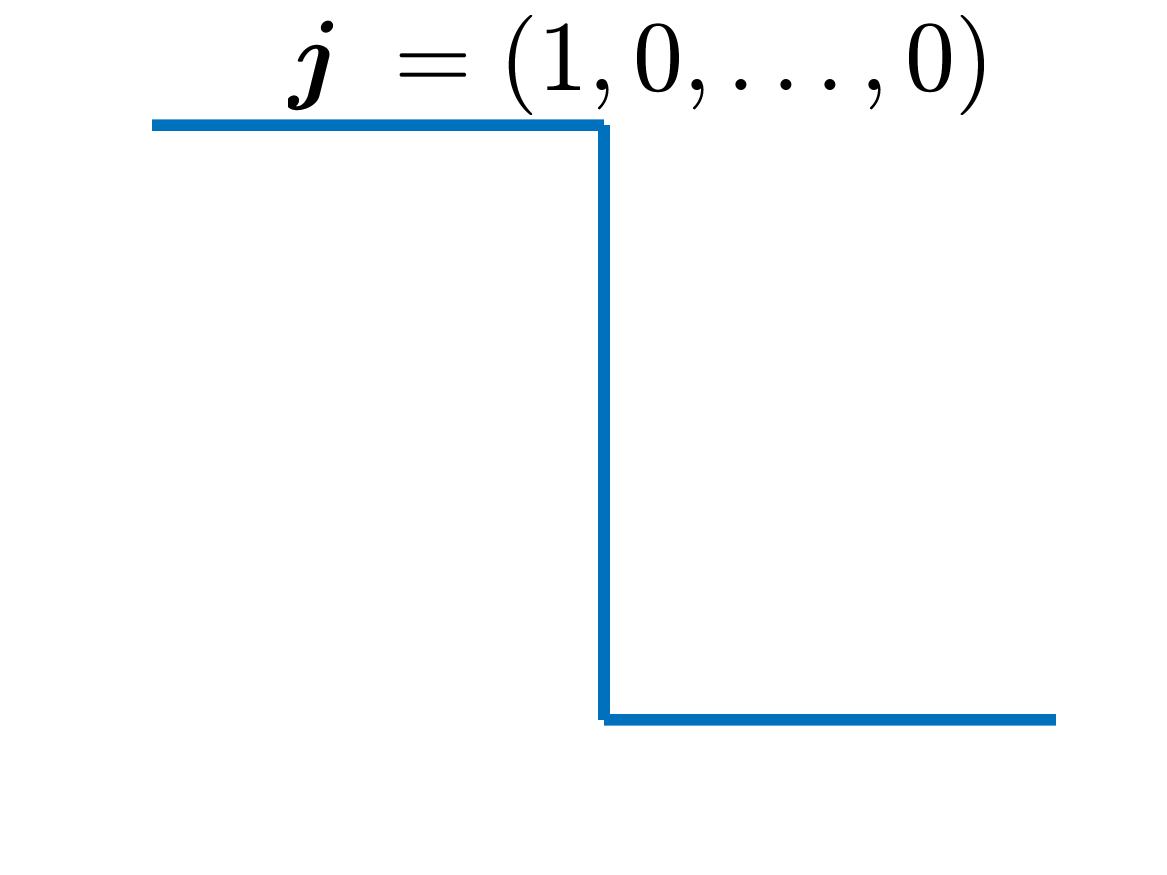
\includegraphics[width =0.18\textwidth]{ProgramsImages/Walsh_Degree_1.png}  &
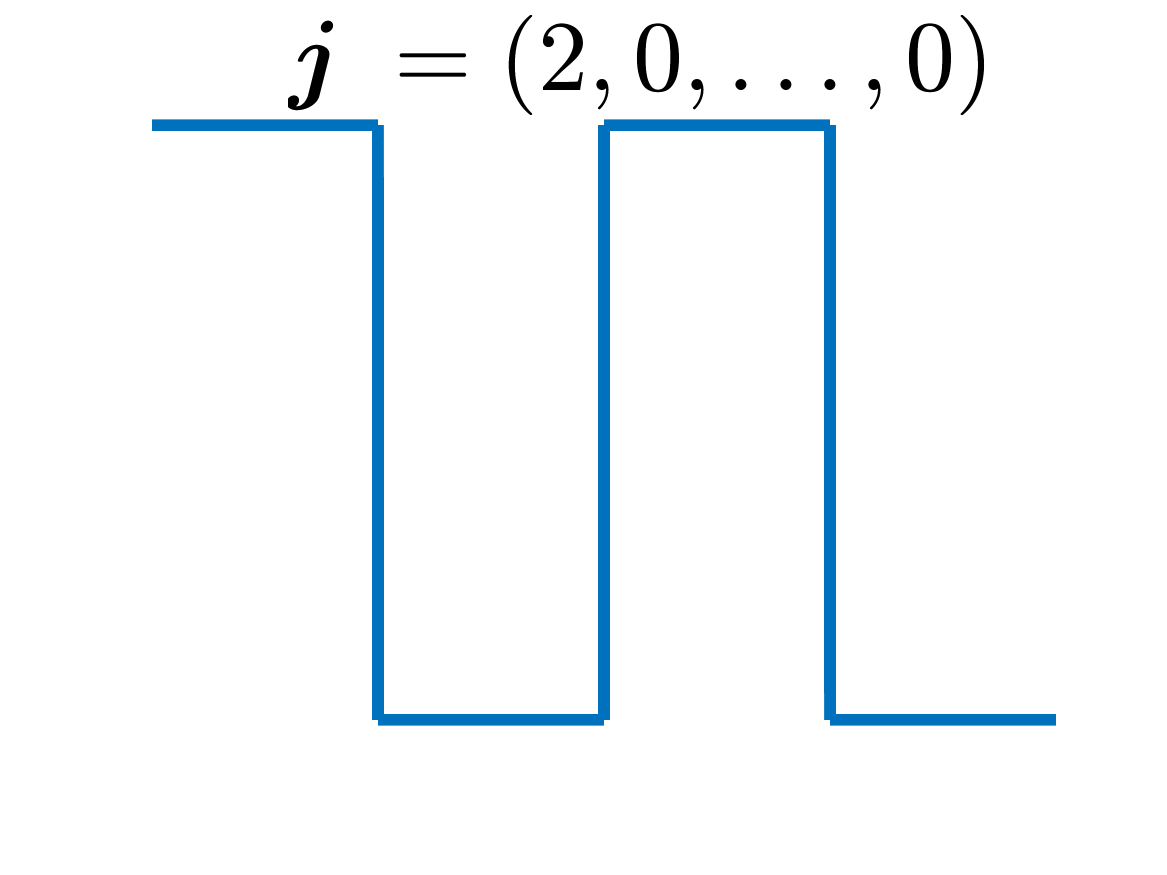
\includegraphics[width =0.18\textwidth]{ProgramsImages/Walsh_Degree_2.png}  &
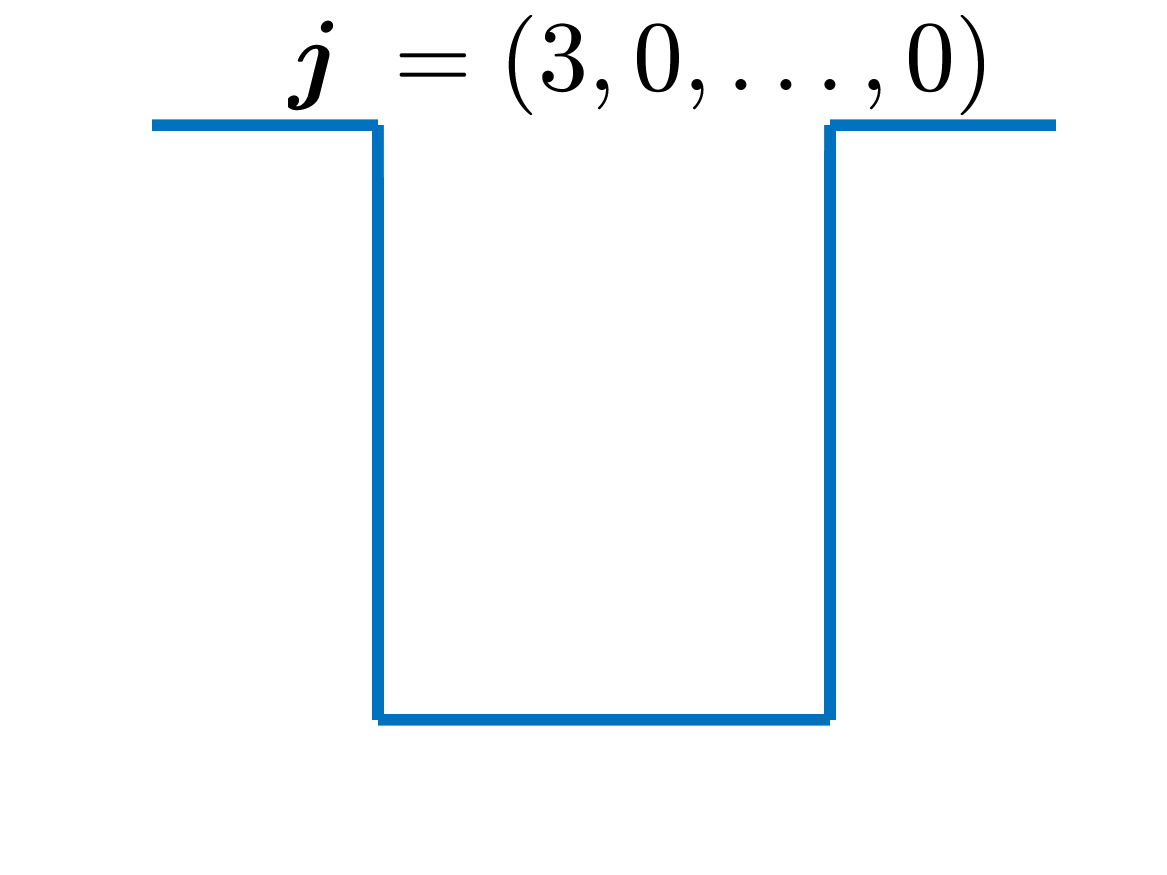
\includegraphics[width =0.18\textwidth]{ProgramsImages/Walsh_Degree_3.png}  &
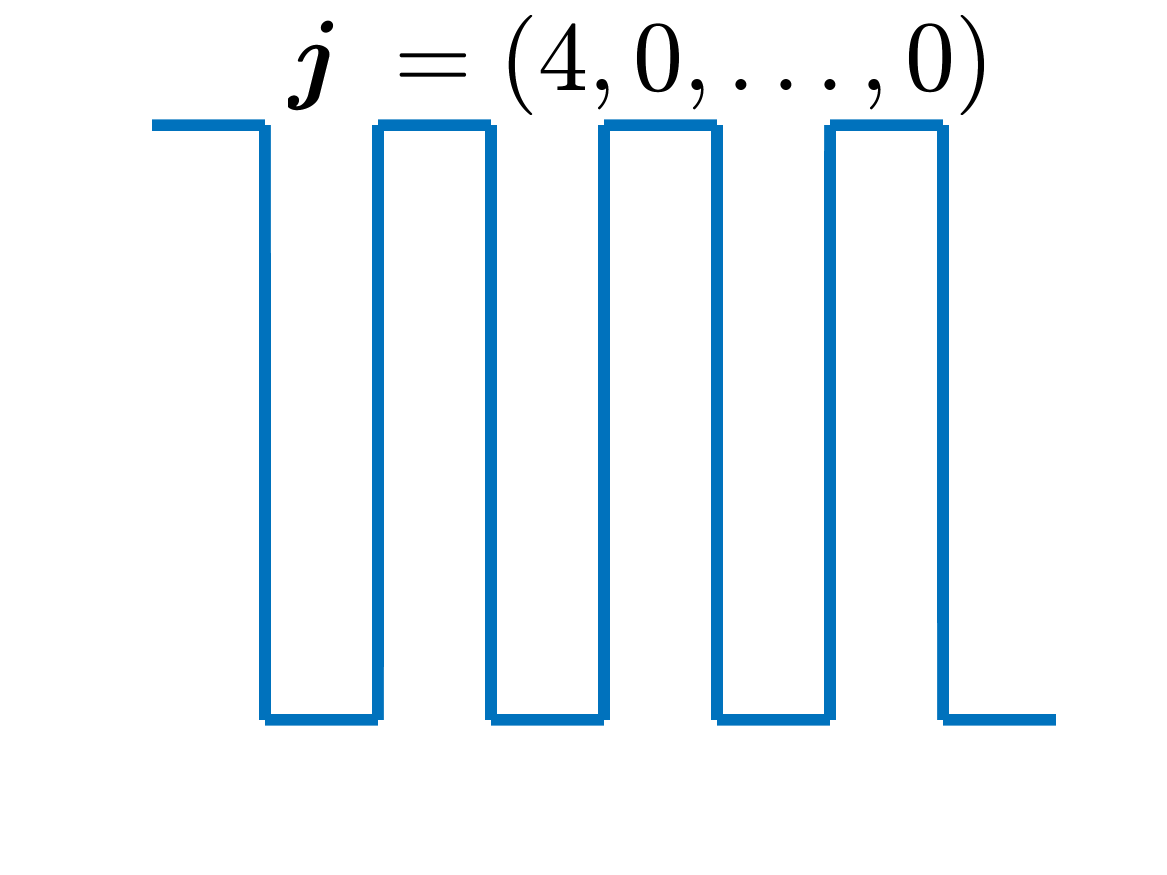
\includegraphics[width =0.18\textwidth]{ProgramsImages/Walsh_Degree_4.png} 
\tabularnewline[-7ex]
Walsh \tabularnewline
\tabularnewline
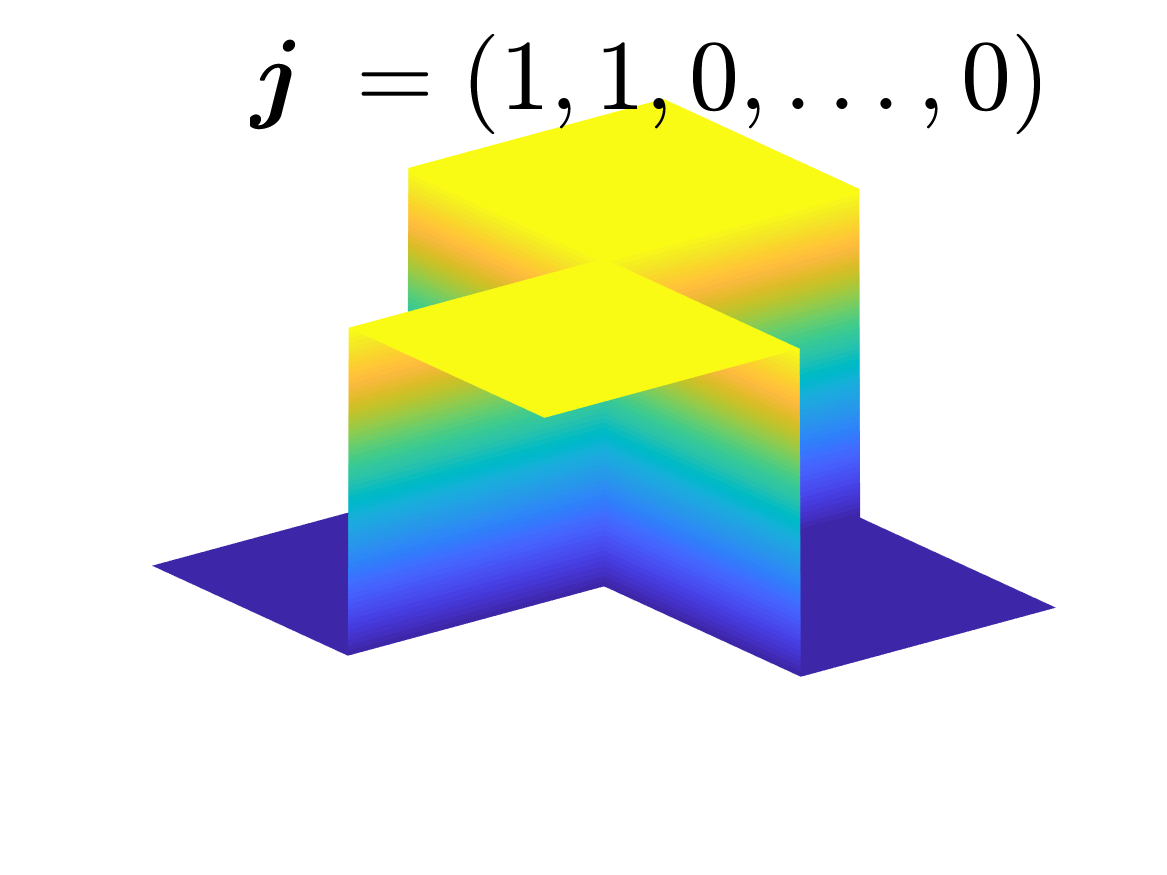
\includegraphics[width =0.18\textwidth]{ProgramsImages/Walsh_Degree_1_1.png}  &
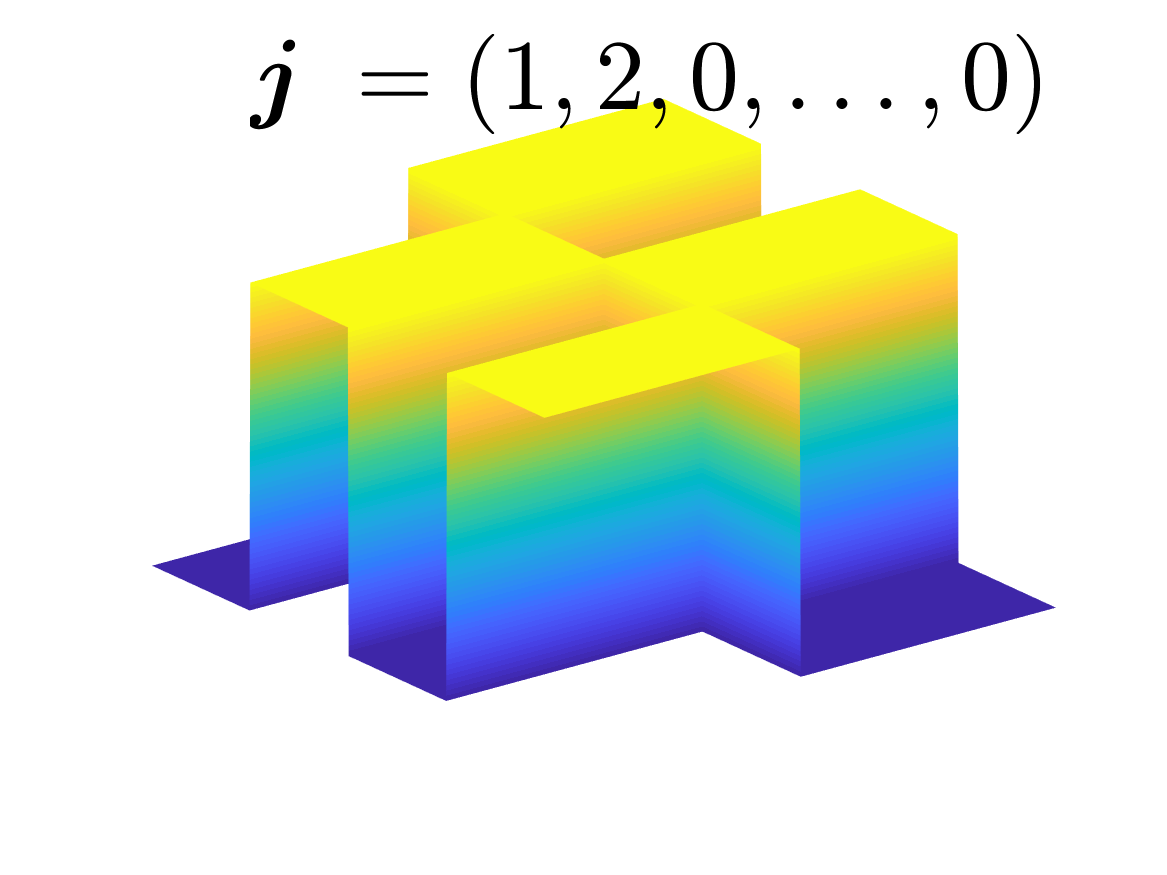
\includegraphics[width =0.18\textwidth]{ProgramsImages/Walsh_Degree_1_2.png}  &
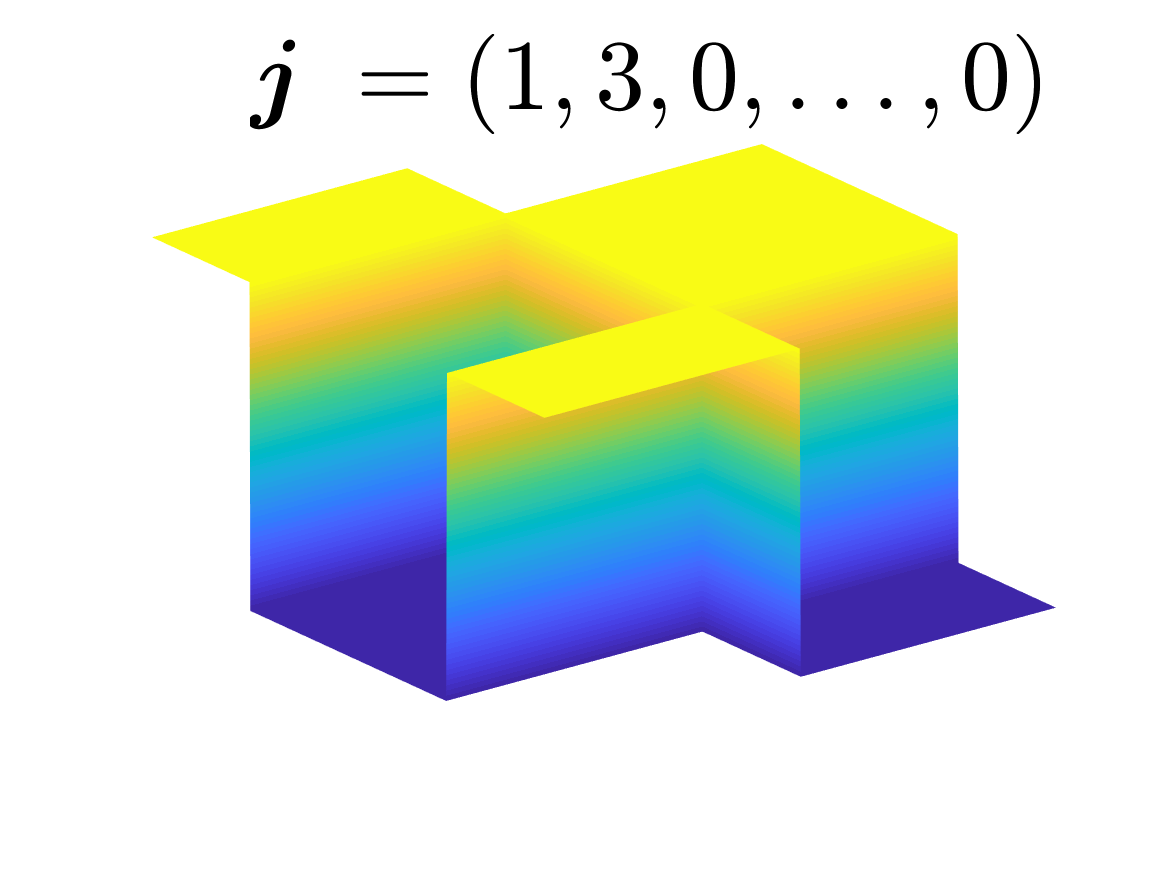
\includegraphics[width =0.18\textwidth]{ProgramsImages/Walsh_Degree_1_3.png}  &
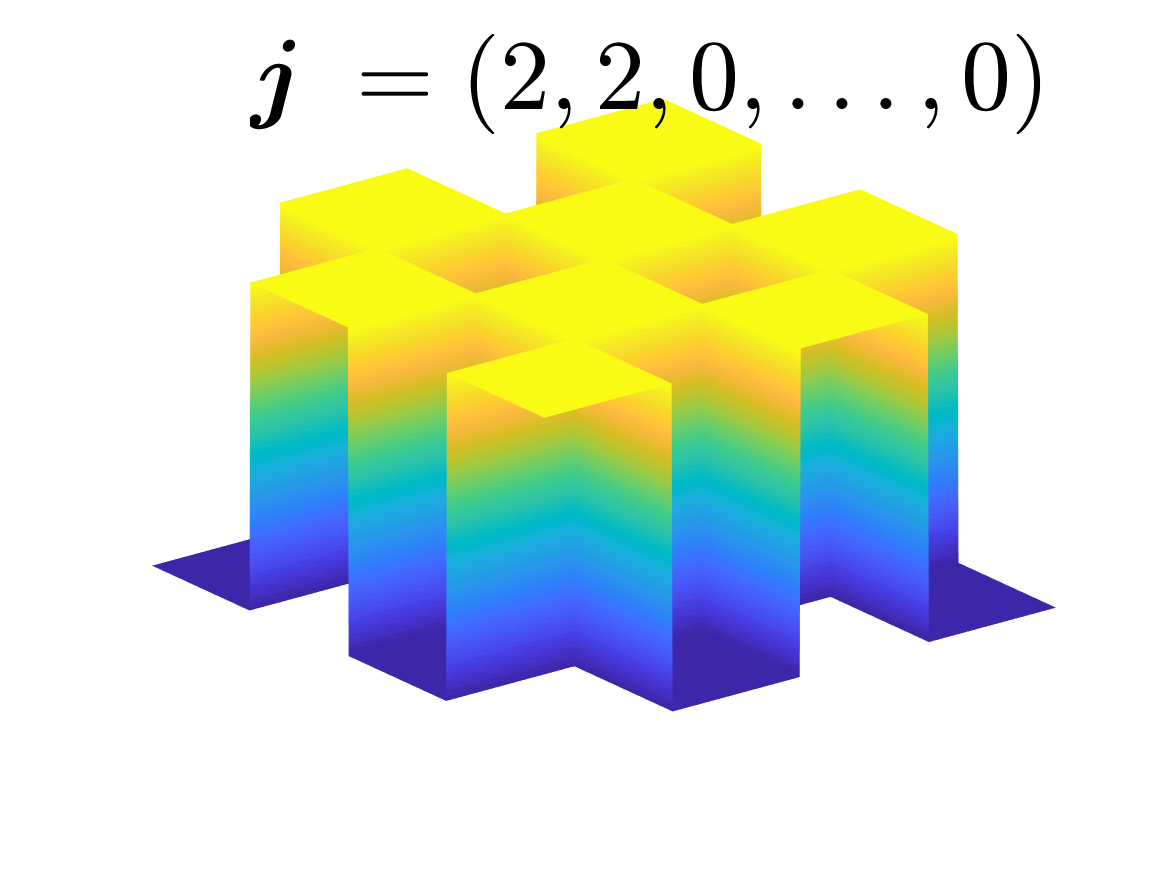
\includegraphics[width =0.18\textwidth]{ProgramsImages/Walsh_Degree_2_2.png}  &
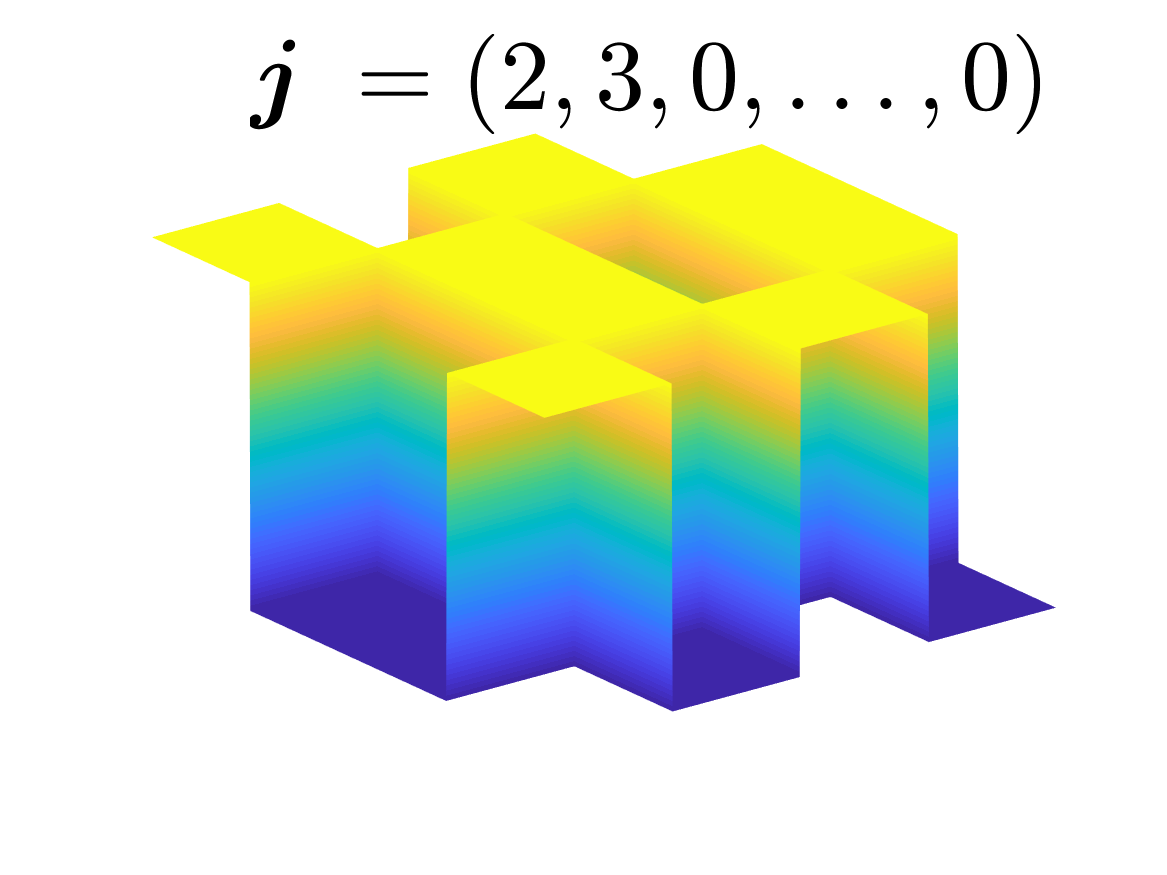
\includegraphics[width =0.18\textwidth]{ProgramsImages/Walsh_Degree_2_3.png} 
	\end{tabular}
\end{frame}


\begin{frame}{Integration Using Function Values \footfullcite{HicJim16a,JimHic16a}}

\vspace{-7ex}

\begin{align*}
    \cf &:= \left \{ f = \sum_{\vj \in \cn} \hf(\vj) u_{\vj} : \norm[\cf]{f} := \bignorm[1,\vlambda]{\hf} : = \norm[1]{\left(\frac{\bigabs{\hf(\vj)}}{\lambda_{\vj}} \right)_{\vj \in \cn}} \right \}\\
    u_{\vj} &= \text{Cosine/Sine or Walsh} \qquad S(u_{\vj}) = \int_{[0,1]^d} u_\vj (\vx) \, \dif \vx = \delta_{\vj,\vzero}, \qquad \cg : = \reals \\
    \Sapp(f,n) &= \frac 1n \sum_{i=1}^n f(\vx_i) = \sum_{\vj \in \text{dual set}} \hf(\vj), \qquad \{\vx_i\}_{i=1}^n = \text{lattice or net} \quad   \\
    &\abs{S(f) - \Sapp(f,n)} \le \sum_{\vzero \ne \vj \in \text{dual set}} \bigabs{\hf(\vj)}
    \quad \includegraphics[width=2cm]{ProgramsImages/SSobolPts.eps}
\end{align*}

\end{frame}



\begin{frame}{Cones that Make Sense for Series Spaces}
\begin{gather*}
    \cf := \left \{ f = \sum_{\vi \in \cn} \hf(\vi) u_{\vi} : \norm[\cf]{f} := \bignorm[q,\vgamma]{\hf} : = \norm[q]{\left(\frac{\bigabs{\hf(\vi)}}{\gamma_{\vi}} \right)_{\vi \in \cn}} \right \} \\
    \cg : = \left \{ g = \sum_{\vi \in \cn} \hg(\vi) v_{\vi} : \norm[\cg]{g} := \bignorm[q']{\hg}\right \}, \qquad S(u_{\vi}) = v_{\vi}, \\
    \text{If } \gamma_{\vi_1} \ge \gamma_{\vi_2} \ge \cdots, \text{ then } \hS_n(f) = \sum_{j=1}^n \hf(\vi_j) v_{\vi_j} \text{ is a good buidling block} \\
    \text{E.g., Function recovery: } S(u_{\vi}) = u_{\vi} = v_{\vi}
\end{gather*}

    
\end{frame}




\thankyouframe

\printbibliography

\section{Bonus}
\begin{frame}[label = VectorSpaceThmProof]{Proof of Theorem for Solvability on a Vector Space}

\vspace{-3ex}

Let the cone $\cc$ be a \alert{vector space} and let

\vspace{-3ex}
\begin{itemize}
    \item $A$ be a successful algorithm
    
    \item $\varepsilon > 0$ be any positive tolerance
    
    \item  $\{L_1, \ldots, L_{M}\} \subset \Lambda$ be the linear functionals used by $A(0,\varepsilon)$, and
    
    \item  $\{L_1, \ldots, L_m\}$ be a basis for $\spann(\{L_1, \ldots, L_{M}\})$
    
    \item $n  = \min(m,\dim(\cc))$
    
        \item $\{f_1, \ldots, f_n\} \subset \cc$ satisfy $L_i(f_j) = \delta_{i,j}$, $i =1, \ldots, n$, $j=1, \ldots, m$
\end{itemize}

\vspace{-2ex}

For any $f \in \cc$, let $\tf = f- \sum_{i=1}^n L_i(f) f_i$, and note that $L_j(\tf) = 0$ for $j =1, \ldots, M$.  Thus, $A(\tf,\varepsilon) = A(0,\varepsilon)$, and so by the \hyperlink{ZeroCorollary}{\beamergotobutton{Corollary}},
\[
0 = S(\tf) = S(f) - \sum_{i=1}^n L_i(f) S(f_i), \qquad \text{which implies } S(f) = \sum_{i=1}^n L_i(f) S(f_i)
\]

\vspace{-3ex}
    \hyperlink{VectorSpaceThm}{\beamerreturnbutton{Back}}
\end{frame}


\begin{frame}[label = BallsWontHelp]{But I Like Balls \smallscoop!}

\vspace{-5ex}
How might you construct an adaptive algorithm if you insist on using \alert{balls}?

\vspace{-2ex}
\begin{description}
    \item[Step 1] Start with a default radius $\rho$, and assume input $f \in \cb_{\rho}$
    
    \item[Step 2] Choose $n$ large enough so that 
    \[
    \norm[\cg]{S(f) - \Sapp(f,n)} \le \varepsilon \qquad \forall f \in \cb_{\rho}, \qquad \text{where } \Sapp(f,n) = \sum_{i=1}^n L_i(f) g_i
    \]
    
    \item[Step 3] Let $\tf \in \cf$ be the \alert{minimum} norm interpolant of the data $L_1(f), \ldots, L_n(f)$.  
    
    \item[Step 4]  If $C\bignorm[\cf]{\tf} \le \rho$ for some preset inflation factor, $C$, then return $A(f,\varepsilon) = \Sapp(f,n)$.  Otherwise, choose $\rho = 2C\bignorm[\cf]{\tf}$, and go to Step 2.
\end{description}

\vspace{-2ex}

This algorithm succeeds for the \alert{cone} \smallcone defined as those functions in $\cf$ whose norms are not much larger than their minimum norm interpolants.   \hyperlink{ConeFrame}{\beamerreturnbutton{Back}}
    
\end{frame}


\end{document}




